\documentclass[11pt,oneside]{book}
\usepackage[a4paper,margin=29mm,headheight=14pt]{geometry}
\usepackage[T1]{fontenc}
\usepackage[utf8]{inputenc}
\usepackage{lmodern}
\usepackage{microtype}
\usepackage{graphicx}
\usepackage{xcolor}
\usepackage{booktabs}
\usepackage{array}
\usepackage{longtable}
\usepackage{tabularx}
\usepackage{enumitem}
\usepackage{amsmath,amssymb,mathtools}
\usepackage{tikz}
\usetikzlibrary{arrows.meta,positioning,fit,shapes.geometric,calc}
\usepackage{listings}
\usepackage{caption}
\usepackage{float}
\usepackage{csquotes}
\usepackage[numbers,sort&compress]{natbib}
\usepackage[hidelinks]{hyperref}
\usepackage{bookmark}
\usepackage{fancyhdr}
\usepackage{titlesec}

\definecolor{ink}{HTML}{17202A}
\definecolor{blue}{HTML}{1F5A85}
\definecolor{teal}{HTML}{167D8D}
\definecolor{pale}{HTML}{EEF5F7}
\definecolor{codebg}{HTML}{F4F6F7}
\definecolor{rulegray}{HTML}{AAB7B8}
\definecolor{covernavy}{HTML}{0B1F33}
\definecolor{coverblue}{HTML}{153E5C}
\definecolor{coverteal}{HTML}{56C6C0}
\definecolor{covercoral}{HTML}{F07B68}
\definecolor{covermist}{HTML}{DCEBED}

\hypersetup{colorlinks=true,linkcolor=blue,citecolor=teal,urlcolor=blue,pdftitle={Designing, Building, and Evaluating Digital Systems},pdfauthor={Scott Brodie Forsyth}}
\setlength{\parindent}{0pt}
\setlength{\parskip}{0.55em}
\setlist{itemsep=0.2em,topsep=0.3em}
\setcounter{tocdepth}{1}

\pagestyle{fancy}
\fancyhf{}
\fancyhead[R]{\small\thepage}
\fancyhead[L]{\small\itshape\nouppercase{\rightmark}}
\renewcommand{\headrulewidth}{0.3pt}

\titleformat{\chapter}[display]
  {\normalfont\bfseries\color{ink}}
  {\filleft\Large\chaptertitlename\ \thechapter}
  {1ex}
  {\Huge\filright}
\titleformat{\section}{\Large\bfseries\color{blue}}{\thesection}{0.7em}{}
\titleformat{\subsection}{\large\bfseries\color{teal}}{\thesubsection}{0.7em}{}

\lstdefinestyle{bookcode}{
  backgroundcolor=\color{codebg},
  basicstyle=\ttfamily\small,
  keywordstyle=\color{blue}\bfseries,
  commentstyle=\color{gray}\itshape,
  stringstyle=\color{teal},
  numbers=left,
  numberstyle=\tiny\color{gray},
  numbersep=8pt,
  frame=single,
  rulecolor=\color{rulegray},
  breaklines=true,
  showstringspaces=false,
  tabsize=4,
  columns=fullflexible
}
\lstset{style=bookcode}

\newcommand{\learningobjectives}[1]{\begin{quote}\textbf{What you will learn.} #1\end{quote}}
\newcommand{\plainlanguage}[1]{\begin{quote}\textbf{In plain language.} #1\end{quote}}
\newcommand{\warningbox}[1]{\begin{quote}\colorbox{pale}{\parbox{0.92\linewidth}{\textbf{Caution.} #1}}\end{quote}}
\newcommand{\exambox}[1]{\begin{quote}\textbf{Project checkpoint.} #1\end{quote}}
\newcommand{\exercise}[1]{\paragraph{Exercise.} #1}
\newcommand{\solution}[1]{\paragraph{Worked solution.} #1}
\newcommand{\term}[1]{\textit{#1}}

\newenvironment{keyterms}{\begin{quote}\textbf{Key terms.}\ }{\end{quote}}


\begin{document}
\frontmatter
\begin{titlepage}
\pagecolor{covernavy}
\thispagestyle{empty}

\sffamily
\vspace*{23mm}
\begin{center}
\begin{minipage}{0.82\textwidth}
  {\small\bfseries\color{coverteal} INFORMATION TECHNOLOGY\hfill 2026 EDITION\par}
  \vspace{15mm}
  {\color{white}\bfseries\fontsize{29}{34}\selectfont
    Designing,\\[-1pt]
    Building, and\\[-1pt]
    Evaluating\\[-1pt]
    {\color{coverteal}Digital Systems}\par}
  \vspace{9mm}
  \textcolor{covercoral}{\rule{0.31\textwidth}{1.4pt}}\par
  \vspace{7mm}
  {\color{covermist}\large
    A principled introduction to information technology,\\
    digitalisation, and application development\par}
  \vspace{9mm}
  {\color{white}\normalsize
    Concepts, methods, and practice for digital systems\par}
  \vspace{7mm}
  {\color{white}\large\bfseries Scott Brodie Forsyth\par}
  \vspace{5mm}
  \textcolor{covercoral}{\rule{0.14\textwidth}{1.4pt}}\par
\end{minipage}
\end{center}

\vfill
\begin{center}
\begin{minipage}{0.82\textwidth}
  \color{covermist}\small
  \textbf{TEXTBOOK EDITION}\hfill Scott Brodie Forsyth\par
  \vspace{2mm}
  \rule{\textwidth}{0.35pt}\par
  \vspace{2mm}
  \scriptsize Information technology, digitalisation, and application development\hfill 2026 edition\par
\end{minipage}
\end{center}
\end{titlepage}
\pagecolor{white}
\color{ink}


\thispagestyle{empty}
\null\vfill
\begin{center}
{\large\bfseries Designing, Building, and Evaluating Digital Systems\par}
\vspace{6mm}
Scott Brodie Forsyth\par
\vspace{6mm}
\textcopyright\ 2026 Scott Brodie Forsyth\par
\vspace{8mm}
This is an independent textbook written for learning, discussion, and practice. It is not affiliated with or endorsed by any university, institution, or organisation.
\end{center}
\vfill\null
\cleardoublepage

\chapter*{Preface}
\addcontentsline{toc}{chapter}{Preface}

Digital systems are made of code, data, interfaces, organisations, and decisions. A program can be syntactically correct and still solve the wrong problem. A database can be fast and still encode a harmful policy. A beautiful interface can be inaccessible. A predictive model can be accurate on a test set and still be unsafe in use. This book is organised around those connections.

The intended reader may arrive from computer science, social science, design, teaching, business, or another discipline. The first chapters therefore begin with ordinary examples and gradually introduce formal language. The aim is not to lower the intellectual level. It is to make the reasoning visible before asking the reader to manipulate its notation.

The scope of this book was inspired by the broad range of questions encountered in a modern information-technology degree, but the book is not a degree programme, course catalogue, or institutional manual. It is a standalone synthesis. Its purpose is to show how ideas from computing, software engineering, interaction design, organisations, research, and artificial intelligence fit together when we try to understand and build digital systems.

One recurring case, CivicQueue, follows a fictional public-service appointment system from an uncertain problem to a tested prototype, a relational database, a deployable web service, an organisational intervention, and a bounded research evaluation. The case is deliberately imperfect. It gives readers opportunities to identify assumptions, privacy risks, competing stakeholder interests, and claims that the evidence cannot support.

The central question is simple: \emph{what must be true for this digital system to be a responsible answer to this problem?} The chapters provide different ways of answering it: computational models, algorithms, software architecture, interaction design, organisational analysis, empirical research, and critical reflection. You can read the book from beginning to end, or enter through the chapter that matches the problem in front of you.

\vfill
\begin{flushright}
July 2026
\end{flushright}

\chapter*{How to use this book}
\addcontentsline{toc}{chapter}{How to use this book}

Each chapter moves from a concrete problem to concepts, formal reasoning, implementation, limitations, and exercises. Read the first explanation quickly, then slow down when the notation or code appears. A useful test of understanding is whether you can explain the idea without repeating the book's example.

The recurring case is not a single prescribed project. Treat it as a laboratory. Replace its public-service setting with a domain you know, but preserve the discipline of stating stakeholders, assumptions, data, interfaces, failure modes, and evidence.

\section*{A practical study loop}
\begin{enumerate}
\item Read the motivating problem and write down what is still unknown.
\item Run the smallest executable example before changing it.
\item Draw the system or model in your own notation.
\item Solve the conceptual exercises without looking at the solutions.
\item Modify the example to violate one assumption and observe the failure.
\item Record the decision, evidence, and limitation in a project log.
\end{enumerate}

The exercises are grouped as conceptual, technical, design, programming, research, and mini-project work. In collaborative work, distribute responsibility for implementation, modelling, user research, testing, and writing, but rotate roles so that everyone can explain the whole system and its limitations.

\warningbox{A passing test suite is evidence about the tested cases. It is not proof that the system is correct in every environment. The same distinction applies to user studies, simulations, and machine-learning evaluations.}

\chapter*{How the book is organised}
\addcontentsline{toc}{chapter}{How the book is organised}

This book is a guided journey through the ideas needed to understand, design, build, and evaluate digital systems. It is not a timetable or a list of institutional requirements. The chapters are arranged so that each part supplies concepts that make the next part easier, while still allowing readers to move directly to a topic that matters to them.

\begingroup
\setlength{\tabcolsep}{4pt}
\begin{longtable}{p{0.20\textwidth}p{0.12\textwidth}p{0.29\textwidth}p{0.29\textwidth}}
\caption{The architecture of the book.}\label{tab:book-map}\\
\toprule
\textbf{Part or focus} & \textbf{Chapters} & \textbf{Central questions} & \textbf{What the reader develops}\\
\midrule
\endfirsthead
\toprule
\textbf{Part or focus} & \textbf{Chapters} & \textbf{Central questions} & \textbf{What the reader develops}\\
\midrule
\endhead
Foundations & 1--4 & What is a digital system? How can a problem be represented computationally? & Problem statements, models, programs, algorithms, and computational reasoning\\
Engineering systems & 5--10 & How can software be designed, implemented, stored, tested, secured, and operated? & Requirements, architecture, code, data, testing, security, and operational judgment\\
People and practice & 11--14 & How do people experience systems, and how do organisations and teams shape them? & Interaction design, evaluation, organisational analysis, agile practice, and collaboration\\
Evidence and independent work & 15--18 & How can claims be investigated, evaluated, and connected to responsible action? & Research design, human-centred AI, experimentation, entrepreneurship, and thesis reasoning\\
Integration projects & 19--20 & What happens when the concepts meet in a complete problem? & A worked case, project ideas, evaluation plans, and final synthesis\\
Appendices and tools & A--D & Which mathematical, technical, and conceptual tools support the main chapters? & Mathematics, Python and Git, reference tables, and a glossary\\
\bottomrule
\end{longtable}
\endgroup

The parts are not prerequisites in the bureaucratic sense, and they are not meant to be completed at a fixed speed. A beginner may read sequentially and run the examples as they appear. An experienced reader may begin with the case study, research chapter, security material, or a specific engineering problem, then return to earlier chapters when a foundation is needed.

\section*{The recurring movement}
The book repeatedly moves through a chain of questions:
\[
\text{problem} \rightarrow \text{model} \rightarrow \text{program} \rightarrow \text{component} \rightarrow \text{system} \rightarrow \text{organisation} \rightarrow \text{evidence}.
\]
This is not a one-way lifecycle. User research can change the problem; production incidents can change the model; organisational constraints can change the architecture; and evidence can show that an intervention did not achieve its intended effect. The purpose of the sequence is therefore not to prescribe a recipe, but to make the connections visible.

\chapter*{Prerequisite bridge}
\addcontentsline{toc}{chapter}{Prerequisite bridge}

This short bridge is for readers who have not studied computer science. You need only ordinary arithmetic, careful reading, and the willingness to test claims.

\section*{Numbers and units}
Computers represent quantities using finite strings of bits. A bit has two possible states, conventionally written 0 and 1. Eight bits form a byte. A kilobyte is used in two different ways: decimal SI usage means 1,000 bytes, while the binary unit kibibyte means 1,024 bytes. Technical writing should state which convention it uses.

\section*{Functions as input-output rules}
In mathematics, a function assigns exactly one output to each allowed input. If $f(x)=2x+1$, then $f(3)=7$. In programming, a function may also change state, perform I/O, raise an exception, or return different results because of time or randomness. The mathematical analogy is useful, but it is not a complete definition of a program function.

\section*{Evidence and uncertainty}
A measurement is an observation produced by a procedure. It can be noisy, biased, incomplete, or affected by the act of measurement. A sample is not automatically representative of a population. A result can be compatible with a hypothesis without proving it. These distinctions reappear in usability studies, organisational evaluation, and machine learning.

\section*{The minimum command-line vocabulary}
The command line is a text interface for starting programs and inspecting files. A command has a current working directory, inputs, outputs, and an exit status. Version control records changes to files over time. The appendix introduces both tools carefully; the early chapters use commands only when they illuminate the program.

\plainlanguage{A technical system is easier to understand when you can state what goes in, what comes out, what changes in between, and what would count as failure. That is the habit this bridge is designed to establish.}



\tableofcontents
\listoffigures
\mainmatter

\part{Foundations: problems, models, and programs}
\chapter{Information technology as a way of shaping action}
\label{ch:it}

\section{A motivating problem}
Imagine a municipality that wants to reduce missed appointments at a public service centre. Someone proposes an app that lets citizens book, reschedule, and receive reminders. The proposal sounds technical, but the problem is not only technical. Are appointments currently missed because people forget, because the booking process is confusing, because transport is unreliable, or because the available times conflict with work? Who may see a citizen's case? What happens when a person has no smartphone? Which employee is responsible when two systems disagree?

The example is the starting point for CivicQueue, the recurring case in this book. The application matters, but so do the policy, the work routines, the data definitions, the interface, the organisational incentives, and the evidence used to decide whether the intervention helped.

\learningobjectives{By the end of this chapter, you should be able to distinguish computer science, software engineering, information systems, HCI, and digitalisation; describe a digital system as a technical and sociotechnical object; identify boundaries, stakeholders, assumptions, and failure modes; and formulate an initial problem statement suitable for a real project.}

\section{The five-minute explanation}
Information technology is the study and practice of using representations, computation, communication, and automated action to support human and organisational purposes. A computer is not the purpose. It is a general mechanism for manipulating representations according to rules.

\plainlanguage{If a paper form is replaced by a web form, that is digitisation: a change in medium. If the organisation changes how cases are allocated, who can act, what evidence is collected, and how citizens participate, that is digitalisation: a change in practice enabled by digital technology. The two often occur together, but they are not the same.}

Four perspectives help us ask different questions:
\begin{description}
\item[Computer science] What can be computed, how can it be represented, and how efficiently and correctly can it be done?
\item[Software engineering] How can a team produce and maintain software that is reliable, secure, usable, and adaptable under constraints?
\item[Information systems] How do technology, people, processes, rules, and organisations combine to create or fail to create value?
\item[Human--computer interaction] How do people understand, use, experience, and appropriate interactive systems, and how should those systems be designed and evaluated?
\end{description}

These are not competing definitions of the same job. They are complementary lenses. A system can be computationally efficient but organisationally useless, socially harmful, or impossible for users with disabilities.

\section{From a problem to a system}
A useful first move is to separate five statements that are often collapsed into one:
\begin{enumerate}
\item \textbf{Situation:} appointments are missed more often than the organisation considers acceptable.
\item \textbf{Interpretation:} reminders and flexible rescheduling may address part of the problem.
\item \textbf{Intervention:} build CivicQueue with a reminder and rescheduling workflow.
\item \textbf{Mechanism:} the workflow reduces forgetting or lowers the cost of changing an appointment.
\item \textbf{Outcome claim:} after adoption, missed appointments decrease without unacceptable exclusion or administrative burden.
\end{enumerate}
The fifth statement is empirical. It cannot be established merely by demonstrating that the application runs.

\begin{figure}[H]
\centering
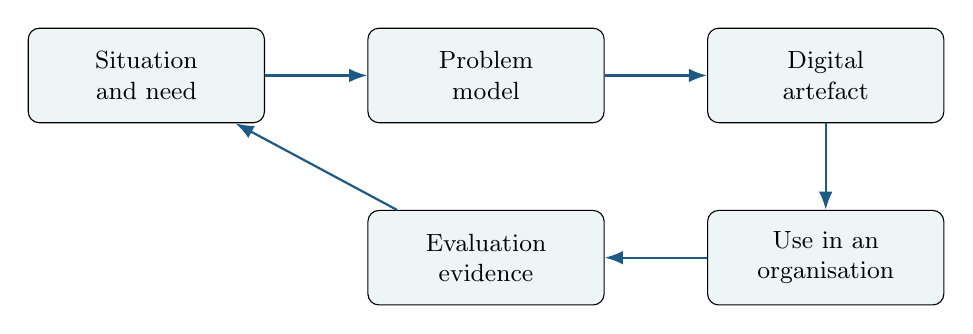
\begin{tikzpicture}[node distance=11mm and 13mm, every node/.style={font=\small}, box/.style={draw, rounded corners, align=center, minimum width=30mm, minimum height=12mm, fill=pale}, arr/.style={-{Latex}, thick, blue}]
\node[box] (situation) {Situation\\and need};
\node[box,right=of situation] (model) {Problem\\model};
\node[box,right=of model] (artefact) {Digital\\artefact};
\node[box,below=of artefact] (use) {Use in an\\organisation};
\node[box,left=of use] (evidence) {Evaluation\\evidence};
\draw[arr] (situation)--(model);
\draw[arr] (model)--(artefact);
\draw[arr] (artefact)--(use);
\draw[arr] (use)--(evidence);
\draw[arr] (evidence)--(situation);
\end{tikzpicture}
\caption{A digital intervention is a cycle of interpretation, construction, use, and evidence.}
\label{fig:it-cycle}
\end{figure}

The arrows in Figure~\ref{fig:it-cycle} are not a rigid waterfall. New evidence can change the problem model; implementation constraints can reveal that the proposed intervention is infeasible; use can produce unexpected workarounds.

\section{A formal vocabulary for boundaries}
For a first approximation, model a system as a tuple
\[
S=(I,O,X,T,R),
\]
where $I$ is a set of inputs, $O$ a set of outputs, $X$ a set of internal states, $T$ a transition rule, and $R$ a set of relevant constraints or requirements. An input might be a request to reschedule. A state might record an appointment and its status. The transition rule determines which state follows a request. An output might be a confirmation page or a message to a staff system.

This model is useful because it forces us to ask what changes and what is observed. It is incomplete because real systems also include people, institutions, physical infrastructure, incentives, and interpretations. In CivicQueue, a transition such as ``appointment confirmed'' is not merely a database update: it may trigger a legal obligation, a staff workflow, and a citizen expectation.

\section{History and intellectual context}
The modern field grew from several traditions: mathematical logic and computation, engineering of reliable artefacts, studies of organisations and information, and research into human action and communication. Turing's analysis of computation helped establish questions about what a machine can do and how we should describe machine behaviour \citep{turing1950computing}. Later, the expansion of networked computing made the boundary between a software product and an organisation increasingly porous.

The history matters because terms such as ``automation'' and ``intelligence'' carry assumptions. A technical system does not become neutral merely because its rules are expressed in code. Choices about categories, defaults, thresholds, and access rights are policy choices as well as implementation choices.

\section{Working example: a bounded problem statement}
An unhelpful project statement is: ``Build an app for appointments.'' It identifies a solution before establishing the problem. A stronger initial formulation is:

\begin{quote}
How can a public-service centre support citizens in changing appointments without telephone contact, while preserving accessibility, privacy, staff control, and a reliable record of appointment status?
\end{quote}

The question is still broad, but it identifies an activity, a context, constraints, and a boundary. It does not promise that a digital channel will reduce missed appointments. That is a claim to investigate.

\subsection{Stakeholders and system boundary}
Primary stakeholders include citizens, front-desk staff, case workers, managers, and system administrators. Secondary stakeholders include accessibility advisers, data-protection officers, the organisation that supplies the calendar service, and people affected by resource allocation but not directly using the app. A boundary diagram should distinguish:
\begin{itemize}
\item the CivicQueue application;
\item external identity, calendar, and notification services;
\item the municipality's case system;
\item people and routines that interpret the outputs.
\end{itemize}

\warningbox{A system boundary is an analytical decision, not a fact discovered in the code. If the boundary excludes the call centre, language support, or the notification provider, the project may hide important causes of failure.}

\section{Professional and ethical responsibility}
The developer's responsibility is not exhausted by implementing the requested feature. Questions include data minimisation, meaningful consent, retention, access control, accessibility, error recovery, vendor dependency, and the consequences of exclusion. The GDPR provides a legal framework for personal-data processing, but compliance is not identical to ethical adequacy \citep{gdpr2016}.

A responsible project makes uncertainty visible. It documents which requirements came from stakeholders, which are assumptions, which are design decisions, and which were evaluated. It gives users a path to recover from mistakes and a human route when the digital path fails.

\section{Using the chapter in a project}
Start a project notebook with four tables:
\begin{enumerate}
\item situation and problem evidence;
\item stakeholder interests and risks;
\item assumptions and open questions;
\item proposed artefacts and evidence needed to evaluate them.
\end{enumerate}
When documenting the work, separate the problem analysis from the solution proposal. When presenting it, be ready to explain why the boundary is reasonable, which stakeholder is missing, and what evidence would change your interpretation.

\section{Summary and key terms}
Information technology joins computation, artefacts, people, and institutions. Computer science, software engineering, information systems, and HCI answer different but connected questions. Digitalisation changes practices and relations, not just file formats. A running application is an intervention, not automatically a solution or a research result.

\begin{keyterms}information technology; digitisation; digitalisation; computer science; software engineering; information systems; HCI; stakeholder; system boundary; sociotechnical system; requirement; intervention; mechanism; outcome.\end{keyterms}

\section{Exercises and worked solutions}
\exercise{Choose a familiar service. Write one sentence describing its situation, one sentence describing a possible intervention, and one sentence describing an outcome that would require evidence.}
\solution{For a library, the situation might be that reserved books are not collected in time. The intervention might be a reminder and cancellation workflow. The outcome claim could be that the proportion of reservations collected within seven days increases without disadvantaging users who do not use email. The three sentences are deliberately different kinds of statement.}

\exercise{Which perspective is most directly concerned with a confusing rescheduling screen: computer science, software engineering, information systems, or HCI? Which other perspectives still matter?}
\solution{HCI is the most direct perspective because it concerns interaction and understanding. Software engineering matters because the screen must be maintainable and integrated with reliable state transitions; computer science matters for the underlying computation; information systems matters because the screen changes a work process and may redistribute responsibility.}

\exercise{Draw the boundary of CivicQueue twice: once narrowly around the web application and once around the complete appointment service. What becomes visible in the second drawing?}
\solution{The wider boundary reveals staff routines, telephone fallback, identity services, notification providers, accessibility support, legal constraints, and the meaning of an appointment status. It also shows that technical success is only one condition for service success.}

\section{Further reading}
For further reading, compare the sociotechnical perspective in \citet{orlikowski1992duality} with the information-systems success model in \citet{delone1992success}, and explore the project-based learning literature if you are working collaboratively.

\chapter{Computational thinking, models, and simulations}
\label{ch:computational-thinking}

\section{A motivating problem}
A city planner asks whether a change in housing allocation could reduce residential segregation. A programmer suggests a simulation in which agents move when too few neighbours are similar to them. The model is simple and often surprising: modest individual preferences can produce large-scale separation. But what exactly does the simulation show? It shows what follows from the rules of that model under its assumptions. It does not, by itself, estimate the effect of a real housing policy.

This chapter develops the habits needed to formulate problems computationally without confusing a model with reality. The same habits support web applications, algorithms, databases, and empirical research.

\learningobjectives{You should be able to decompose a problem, identify abstractions and state variables, describe deterministic and stochastic transitions, implement a reproducible agent-based simulation, distinguish verification from validation, and discuss sensitivity and model limitations.}

\section{The five-minute explanation}
Computational thinking is a family of problem-solving practices: decomposition, abstraction, representation, algorithm design, automation, and evaluation. It is not the claim that every problem should be reduced to code. It is a disciplined way to ask which parts of a problem can be represented by rules and which parts remain uncertain, normative, or outside the model.

\plainlanguage{A model is a deliberately simplified answer to the question \enquote{what features do we need to keep in order to study this behaviour?} Removing detail can make a model usable, but every removal is an assumption.}

\section{Decomposition and representation}
Suppose CivicQueue must support rescheduling. Decompose it into smaller questions:
\begin{enumerate}
\item What counts as an appointment?
\item Which states can an appointment have?
\item Who may request a change?
\item Which time slots are available?
\item What happens when two requests arrive together?
\item Which systems and people must be notified?
\end{enumerate}
This decomposition creates representations: a state machine, a data model, access-control rules, and a sequence of interactions. Different representations make different errors easy to see.

\section{State and transition systems}
Let $X$ be a set of states and $A$ a set of actions. A deterministic transition function is
\[
T:X\times A\rightarrow X.
\]
The notation says that, for a current state $x\in X$ and an action $a\in A$, the system produces one next state $T(x,a)$. If an action is not allowed, the transition is undefined or produces an error state. A stochastic transition can instead be written as a probability distribution $P(x'\mid x,a)$ over possible next states.

For an appointment, let $X=\{\text{requested},\text{confirmed},\text{cancelled},\text{completed}\}$. An invariant might be that a cancelled appointment cannot become completed without a new appointment being created. The invariant is a claim about all allowed transitions, not merely an example trace.

\begin{figure}[H]
\centering
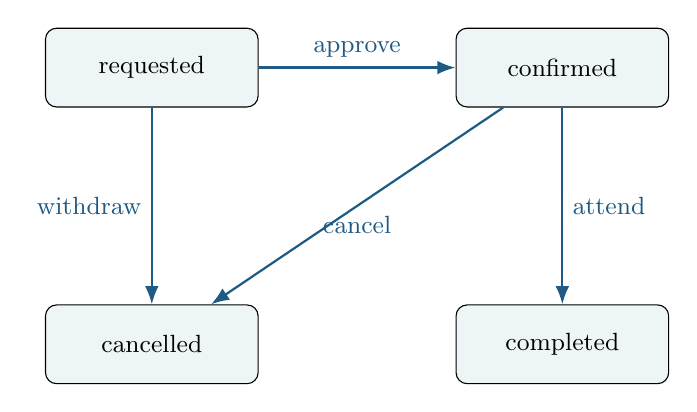
\begin{tikzpicture}[node distance=25mm, every node/.style={font=\small}, state/.style={draw, rounded corners, fill=pale, minimum width=27mm, minimum height=10mm}, arr/.style={-{Latex}, thick, blue}]
\node[state] (requested) {requested};
\node[state,right=of requested] (confirmed) {confirmed};
\node[state,below=of confirmed] (completed) {completed};
\node[state,below=of requested] (cancelled) {cancelled};
\draw[arr] (requested)--node[above]{approve}(confirmed);
\draw[arr] (confirmed)--node[right]{attend}(completed);
\draw[arr] (requested)--node[left]{withdraw}(cancelled);
\draw[arr] (confirmed)--node[below]{cancel}(cancelled);
\end{tikzpicture}
\caption{A small appointment state machine. An omitted transition is not automatically permitted.}
\label{fig:appointment-state}
\end{figure}

\section{Agent-based models}
In an agent-based model, individual entities follow local rules while a simulation records the resulting system-level pattern. A minimal segregation model places agents on a grid. Each agent has a type, a neighbourhood, and a tolerance threshold. At each step, an unhappy agent moves to an empty location where its local condition is satisfied.

The model's main variables are:
\begin{itemize}
\item grid size and occupancy;
\item agent types;
\item neighbourhood definition;
\item tolerance threshold;
\item update order;
\item random seed;
\item stopping rule.
\end{itemize}

Changing any one can change the result. A random seed makes one run reproducible; it does not make a random process deterministic in the world.

The implementation in \texttt{examples/simulation/segregation.py} uses only the Python standard library. It returns a result object rather than printing from the model, which makes it easier to test and reuse.

\begin{lstlisting}[language=Python,caption={A small transition rule from the simulation.}]
def is_happy(grid, row, col, tolerance):
    """Return whether the occupied cell satisfies its local rule."""
    agent = grid[row][col]
    if agent is None:
        return True
    neighbours = neighbours_of(grid, row, col)
    occupied = [item for item in neighbours if item is not None]
    if not occupied:
        return True
    similar = sum(item == agent for item in occupied)
    return similar / len(occupied) >= tolerance
\end{lstlisting}

The function does not claim that similarity is a complete description of social satisfaction. It is a formalisation chosen for a particular experiment.

\section{Verification, validation, and sensitivity}
\term{Verification} asks whether the implementation follows the specified model. Tests can check that an empty neighbourhood makes an agent happy, that no agent moves when all agents are happy, and that the same seed produces the same trace. \term{Validation} asks whether the model is an adequate representation for a purpose. That requires substantive argument and possibly comparison with data or expert knowledge.

For a parameter $\theta$, a sensitivity analysis examines how an outcome $Y$ changes when $\theta$ changes. A simple finite-difference measure is
\[
\Delta Y = Y(\theta+\delta)-Y(\theta),
\]
where $\delta$ is a specified change. The quantity is meaningful only when the outcome, parameter range, randomisation procedure, and comparison are stated. If results change dramatically under plausible values, conclusions should be conditional rather than absolute.

\warningbox{A simulation can be internally correct and externally irrelevant. A realistic-looking animation is not evidence of validation. State the target phenomenon, the purpose of the model, and the assumptions that connect the model to that phenomenon.}

\section{Other computational models}
Conway's Game of Life uses a local rule on a grid and demonstrates emergence: global patterns arise from repeated local transitions. Flocking models represent agents with rules for separation, alignment, and cohesion. Epidemic models represent contact and transmission. Network diffusion represents entities as nodes and relations as edges. Schelling-style models represent local preferences and movement. These examples teach formalisation and emergent behaviour, but they should not be presented as direct explanations of human society.

\section{Parameters and experimental design}
An experiment is easier to interpret when it changes one planned factor at a time or uses a documented factorial design. Record:
\begin{enumerate}
\item the research or modelling question;
\item the outcome measure and its units;
\item parameter values and ranges;
\item number of replications;
\item random seeds;
\item software version and environment;
\item analysis procedure and stopping rules.
\end{enumerate}
Reproducibility is not the same as truth. It is a condition for checking the reasoning that produced a result.

\section{Project application}
For a computational-thinking project, begin with a problem from a domain you understand. Define the target phenomenon before selecting a technique. Include a model diagram, a table of variables, pseudocode, implementation tests, at least one sensitivity analysis, and a section called \enquote{What this model cannot establish.} When presenting the work, be prepared to change a parameter or rule and explain why the interpretation changes.

\section{Summary and key terms}
Computational thinking makes choices about decomposition, representation, and automation explicit. State-transition models support reasoning about software. Agent-based models can reveal emergence from local rules. Verification concerns implementation against a specification; validation concerns adequacy for a purpose. Random seeds, sensitivity analysis, and documented parameters support reproducibility and honest interpretation.

\begin{keyterms}computational thinking; abstraction; representation; state; transition; invariant; deterministic; stochastic; agent-based model; emergence; verification; validation; sensitivity analysis; reproducibility.\end{keyterms}

\section{Exercises and worked solutions}
\exercise{Write an invariant for CivicQueue's appointment states and give one invalid transition.}
\solution{One invariant is that an appointment marked completed must have previously been confirmed. An invalid transition is cancelled $\rightarrow$ completed. A legitimate new booking after cancellation should create a new appointment identifier rather than silently changing the old record.}

\exercise{Why does a random seed help a simulation study? What does it not do?}
\solution{It makes a particular pseudo-random sequence reproducible, allowing a reviewer to rerun the same case. It does not remove uncertainty, guarantee that the seed is representative, or validate the model.}

\exercise{Design a sensitivity analysis for the segregation model.}
\solution{Choose a tolerance range, for example 0.3 to 0.8, specify grid size and occupancy, run multiple seeds at each value, and report the mean and variation of a pre-defined segregation measure. Do not change the stopping rule or outcome definition between parameter values without documenting it.}

\section{Further reading}
Computational thinking connects algorithm design, abstraction, automation, data representation, and agent-based formalisation. For algorithmic foundations, see \citet{cormen2022introduction}; for the relation between models and computation, see \citet{abelson1996structure}.

\chapter{Programming from first principles}
\label{ch:programming}

\section{A motivating problem}
Suppose a staff member asks for a script that lists appointments occurring tomorrow. A first attempt might appear to work on a small sample, but a real system must also handle time zones, missing data, invalid dates, duplicate records, permissions, and tests. Programming is the activity of expressing a procedure so that a computer can execute it. Good programming also requires making assumptions, boundaries, and failure behaviour explicit.

\learningobjectives{You should be able to explain how source code reaches execution, use Python values and control flow correctly, design functions with clear contracts, handle errors, work with files and structured data, and write tests that expose assumptions.}

\section{The five-minute explanation}
A program is a sequence of instructions interpreted by a runtime or translated by a compiler into a lower-level representation. Python source is parsed into an internal representation and executed by the Python runtime. The exact implementation varies, but the enduring ideas are source text, syntax, semantics, state, control flow, and effects.

\plainlanguage{A variable is not a labelled box containing a string of characters. In Python it is a name bound to an object. Assignment changes a binding; mutation changes an object. Keeping those ideas separate prevents many bugs.}

\section{Values, names, and types}
Python values include integers, floating-point numbers, booleans, strings, lists, dictionaries, and user-defined objects. A type describes the operations and representation available for values of a kind. Python checks many type constraints at runtime; static type checkers can detect additional inconsistencies before execution.

\begin{lstlisting}[language=Python,caption={Bindings, mutation, and a type-annotated function.}]
def add_fee(amount: float, fee: float) -> float:
    if amount < 0 or fee < 0:
        raise ValueError("amounts must be non-negative")
    return amount + fee

first = ["requested"]
second = first
second.append("confirmed")
assert first == ["requested", "confirmed"]
\end{lstlisting}

The two names refer to the same list object. If independent lists are needed, create a copy with \texttt{first.copy()}. An assertion expresses an assumption that should remain true at that point in the program.

\section{Expressions and control flow}
An expression produces a value. A statement performs an action such as assignment, branching, looping, or returning. A conditional is a choice between paths. A loop repeats a block while a condition holds or for each element of an iterable. The important question is not how many keywords a language has, but which control-flow graph the program creates.

\begin{lstlisting}[language=Python,caption={Filtering appointments with an explicit predicate.}]
def confirmed_for_day(appointments: list[dict], day: str) -> list[dict]:
    """Return confirmed appointments whose ISO date equals day."""
    return [
        appointment
        for appointment in appointments
        if appointment.get("status") == "confirmed"
        and appointment.get("date") == day
    ]
\end{lstlisting}

The function uses a list comprehension, but the same logic can be written as a loop. Choose the form that makes the invariant and failure behaviour clearest to the team.

\section{Functions as contracts}
A function should have a small purpose, named inputs, a documented output, and an explicit error policy. A contract can be described as:
\[
\{P\}\;C\;\{Q\},
\]
where $P$ is a precondition, $C$ is the command or function, and $Q$ is a postcondition. For \texttt{add\_fee}, $P$ is that both inputs are non-negative numbers; $Q$ is that the returned value equals their sum and is non-negative. A contract does not make a function correct automatically. It makes the claim inspectable and testable.

\section{Input, output, and files}
External input is untrusted and may be absent, malformed, stale, or malicious. Parse it at the boundary, validate it, and convert it to an internal representation. JSON is a data interchange format, not a security boundary. Never treat data from a request as executable code.

\begin{lstlisting}[language=Python,caption={Safe JSON loading at a file boundary.}]
import json
from pathlib import Path

def load_records(path: Path) -> list[dict]:
    with path.open(encoding="utf-8") as handle:
        data = json.load(handle)
    if not isinstance(data, list):
        raise ValueError("expected a JSON array")
    if not all(isinstance(item, dict) for item in data):
        raise ValueError("every record must be a JSON object")
    return data
\end{lstlisting}

Use context managers so files close even if parsing raises an exception. Validate the shape before using fields. In a production service, add limits on file size and record count.

\section{Errors, exceptions, and debugging}
An error is a mismatch between the program's assumptions and the current situation. Exceptions are one mechanism for transferring control to an error handler. Catch exceptions at a boundary where recovery is possible; do not catch every exception and silently continue. A useful debugging report records the smallest input that reproduces the problem, expected behaviour, actual behaviour, and the first violated assumption.

\section{Testing and executable examples}
The examples directory contains tests alongside the code. A unit test checks a small behaviour in isolation; an integration test checks interactions among components; an end-to-end test follows a user-visible path. Tests are executable claims. They do not remove the need for inspection, threat modelling, accessibility evaluation, or exploratory testing.

\begin{lstlisting}[language=Python,caption={A small test for the appointment filter.}]
def test_confirmed_for_day_ignores_other_statuses():
    rows = [
        {"status": "confirmed", "date": "2026-09-01"},
        {"status": "cancelled", "date": "2026-09-01"},
        {"status": "confirmed", "date": "2026-09-02"},
    ]
    assert confirmed_for_day(rows, "2026-09-01") == [rows[0]]
\end{lstlisting}

The test is precise about status and date. It does not test time zones, malformed records, or permissions; those belong in further tests.

\section{Web foundations}
HTML represents document structure; CSS describes presentation; JavaScript can manipulate the Document Object Model and respond to browser events. HTTP carries requests and responses between clients and servers. A browser event may trigger a request, which invokes server logic, changes persistence, returns a response, and produces visible feedback. Chapter~\ref{ch:web} develops the full path.

\section{Code quality and security}
Readable names, small functions, consistent formatting, dependency control, and version history reduce the cost of reasoning. Security is a property of the whole system: input validation, authentication, authorisation, secrets management, logging, dependency updates, and safe defaults must be designed together. OWASP's Top 10 is a useful awareness list, not a complete security specification \citep{owasptop10}.

\section{Project application}
Start a project with a small vertical slice: one user action, one domain rule, one persistence operation, one visible result, and one test. This makes integration risks visible early. When documenting the work, show the requirements traceability from user need to function to test. When presenting it, explain which code is deliberately simple and what would change for production.

\section{Summary and key terms}
Programming combines representation, control flow, state, functions, effects, and error handling. Names refer to values; mutation and rebinding differ. Contracts express assumptions. Tests provide executable evidence about specified behaviours. Secure and maintainable code requires boundary validation, clear ownership, and feedback from execution.

\begin{keyterms}source code; runtime; value; object; binding; type; expression; statement; control flow; function; scope; precondition; postcondition; invariant; exception; test; module; dependency; API.\end{keyterms}

\section{Exercises and worked solutions}
\exercise{What is the difference between \texttt{second = first} and \texttt{second = first.copy()} when \texttt{first} is a list?}
\solution{The first assignment creates a second name for the same list, so mutation through either name is visible through both. \texttt{copy()} creates a new list with the same current elements, so appending to one list does not append to the other. Nested mutable objects require a deeper copy if independent nested state is needed.}

\exercise{Write a contract for a function that reserves an appointment slot.}
\solution{A possible precondition is that the slot exists, is in the future, and the caller is authorised. The postcondition is that exactly one reservation is created and the slot is no longer available, or that the operation returns a well-defined conflict without changing state. Concurrency means the postcondition must hold even when two requests arrive together.}

\exercise{Name three tests that the appointment filter still needs beyond the example.}
\solution{Tests could cover an empty input, a missing \texttt{status} field, a malformed date, duplicate records, and a date with no confirmed appointments. The correct selection depends on the contract and threat model; a test is useful only when its expected behaviour is justified.}

\section{Further reading}
Good programming practice connects computational thinking, data structures, functions, web basics, testing, and the evaluation of programming solutions. For a gentle introduction, see \citet{downey2015think}; the Python documentation is the reference for language behaviour \citep{pythonlanguage}.

\chapter{Algorithms, data structures, and formal reasoning}
\label{ch:algorithms}

\section{A motivating problem}
CivicQueue may store 100 appointments today and ten million historical records next year. A search that feels instant on a laptop can become unusable at scale. Choosing an algorithm and data structure is therefore a design decision about time, memory, correctness, and future change.

\learningobjectives{You should be able to use sets, relations, functions, sequences, trees, and graphs; explain invariants and induction; implement common data structures; analyse time and space asymptotically; and distinguish asymptotic reasoning from measured performance.}

\section{Sets, relations, and functions}
A set is a collection of distinct elements. If $A=\{1,2,3\}$, then $2\in A$ means 2 is a member. A relation $R$ between sets $A$ and $B$ is a set of ordered pairs from $A\times B$. A function $f:A\to B$ is a relation with exactly one output in $B$ for each input in $A$.

These ideas appear in systems. Let $U$ be users and $P$ be permissions. A relation \texttt{can\_access} \(\subseteq U\times P\) records grants. It may not be a function: one user can have several permissions, and several users can share one permission. Confusing a relation with a function causes bad data models and incorrect code.

\section{Data structures as representations}
An array provides indexed access. A stack supports last-in, first-out operations. A queue supports first-in, first-out operations. A hash table maps keys to buckets using a hash function. A tree represents hierarchy; a graph represents arbitrary relationships.

\begin{figure}[H]
\centering
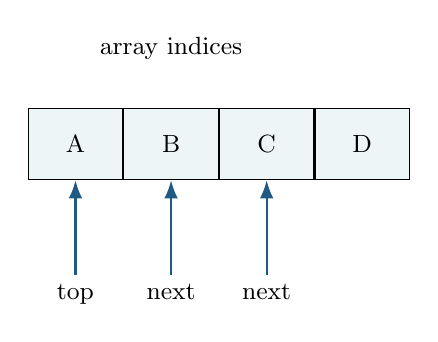
\begin{tikzpicture}[every node/.style={font=\small}, cell/.style={draw, minimum width=12mm, minimum height=9mm, fill=pale}, arr/.style={-{Latex}, thick, blue}]
\node[cell] (a) at (0,0) {A};\node[cell,right=0pt of a] (b) {B};\node[cell,right=0pt of b] (c) {C};\node[cell,right=0pt of c] (d) {D};
\node[above=5mm of b] {array indices};
\node[below=12mm of a] (s1) {top};\node[below=12mm of b] (s2) {next};\node[below=12mm of c] (s3) {next};
\draw[arr] (s1)--(a);\draw[arr] (s2)--(b);\draw[arr] (s3)--(c);
\end{tikzpicture}
\caption{A sequence can support several abstract data types, but the operations and invariants differ.}
\label{fig:data-structures}
\end{figure}

An abstract data type specifies allowed operations and their meaning without fixing an implementation. A queue can be implemented by a list, a linked structure, or a concurrent service. The abstraction helps clients depend on behaviour rather than representation.

\section{Correctness through invariants}
An invariant is a proposition that is true before and after every operation that preserves the data structure. For a queue, an invariant might be that the front element is the oldest element not yet removed. To reason about a loop, identify:
\begin{enumerate}
\item the invariant before the first iteration;
\item why one iteration preserves it;
\item what the invariant implies when the loop stops.
\end{enumerate}
This is a practical form of proof. It can be applied to a cursor in a database query, a parser, or a simulation update.

\section{Induction and recursion}
Mathematical induction proves a statement for all natural numbers. First prove the base case. Then assume it holds for an arbitrary $n$ and prove it holds for $n+1$. Recursive programs use a related structure: a base case and a recursive case that reduces the problem to a smaller instance. A recursive function without a reachable base case does not terminate.

For the sum $1+2+\cdots+n$, define $S(0)=0$ and $S(n)=n+S(n-1)$. The recurrence makes the reasoning explicit. An iterative implementation may be preferable in Python when recursion depth is large.

\section{Searching and sorting}
Linear search checks elements one by one. If the target is equally likely to be anywhere, its average number of comparisons is approximately $(n+1)/2$ when it exists and $n$ when it does not. Binary search repeatedly halves a sorted search interval. Its logarithmic behaviour depends on the precondition that the data is sorted and that the index operation is efficient.

Sorting algorithms illustrate trade-offs. Insertion sort is simple and useful for small or nearly sorted inputs. Merge sort offers $O(n\log n)$ worst-case time and uses extra space. Quicksort is often fast in practice but can have $O(n^2)$ worst-case time unless the pivot strategy and input assumptions are controlled. A library implementation may be preferable because it has been engineered and tested across cases.

\section{Asymptotic notation}
We write $f(n)\in O(g(n))$ if there are constants $c>0$ and $n_0$ such that
\[
0\le f(n)\le c\,g(n) \quad \text{for every }n\ge n_0.
\]
The variable $n$ measures input size. The notation describes an eventual upper bound up to constant factors. It ignores constant costs, hardware, cache behaviour, interpreter overhead, and distribution of inputs. Therefore $O(n)$ is not automatically faster than $O(n\log n)$ for small $n$, and the label does not predict latency without a cost model.

Space complexity applies the same idea to additional memory. A streaming algorithm may use $O(1)$ extra space while taking $O(n)$ time. A hash table may offer expected $O(1)$ lookup under assumptions about hashing and load, while requiring $O(n)$ storage.

\begin{figure}[H]
\centering
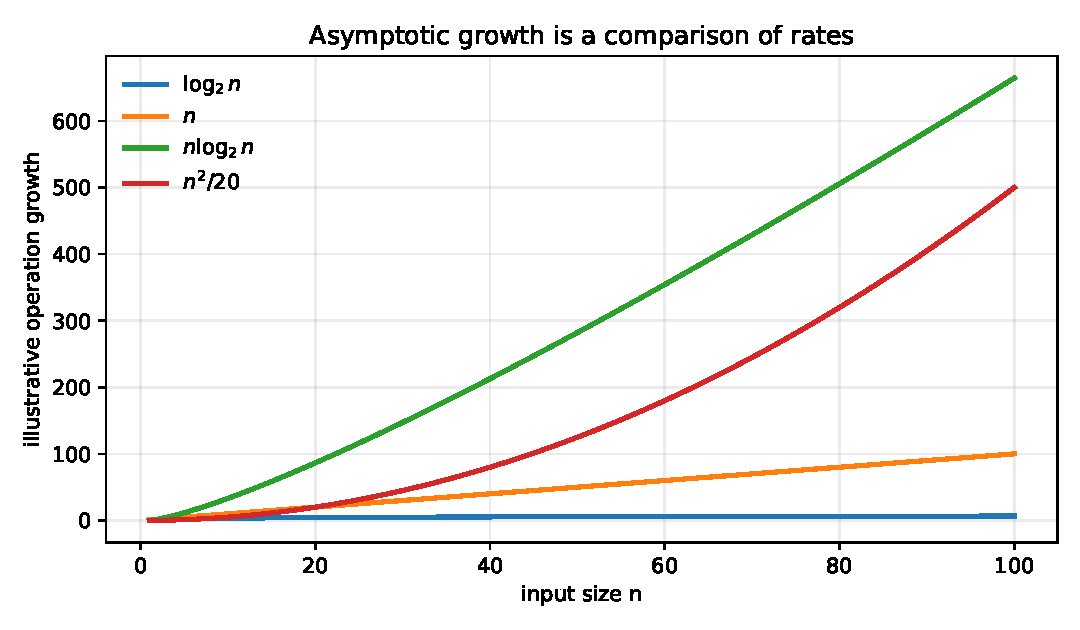
\includegraphics[width=0.78\linewidth]{figures/complexity-plot.pdf}
\caption{Illustrative growth curves generated by \texttt{figures/complexity\_plot.py}. The plot is a teaching aid, not a benchmark.}
\label{fig:complexity}
\end{figure}

\section{Graphs and networks}
A graph $G=(V,E)$ consists of vertices $V$ and edges $E$. Edges may be directed or undirected and may carry weights. In CivicQueue, a graph could represent dependencies among services, escalation paths, or relations among organisations. Breadth-first search explores by distance in an unweighted graph; Dijkstra's algorithm solves shortest paths when edge weights are non-negative. The representation and query determine which algorithm is appropriate.

\section{Measured performance}
Asymptotic analysis and measurement answer different questions. A benchmark should state hardware, software version, input generation, warm-up, repetitions, timing method, and variability. Avoid measuring a toy implementation and generalising to a production system. Profile before optimising; a theoretically elegant algorithm cannot compensate for a database query that returns unnecessary rows or a network call made inside a loop.

\section{Project application}
For any non-trivial feature, record the data structure, operation costs, input-size assumptions, and correctness invariant. When documenting the work, justify the choice in relation to the problem rather than listing Big-O labels. When presenting it, explain a failure case: an unsorted input to binary search, a hash collision, a disconnected graph, or an unexpectedly large recursion depth.

\section{Summary and key terms}
Formal structures clarify what data means. Algorithms are procedures with preconditions, operations, and correctness claims. Invariants and induction provide reusable reasoning tools. Asymptotic notation describes growth under explicit assumptions; measurement is still needed for engineering decisions.

\begin{keyterms}set; relation; function; sequence; abstract data type; array; stack; queue; hash table; tree; graph; invariant; induction; recursion; sorting; searching; asymptotic notation; scalability.\end{keyterms}

\section{Exercises and worked solutions}
\exercise{A list contains 1,000,000 user identifiers. When is a set a better representation than a list?}
\solution{If the main operation is membership testing and order is not required, a set usually offers expected constant-time membership rather than linear scanning. It uses additional memory and depends on hash behaviour. If stable ordering or duplicate values matter, another representation may be more suitable.}

\exercise{State the loop invariant for a linear search that has examined positions $0$ through $i-1$.}
\solution{The target is not present in positions $0$ through $i-1$, unless the algorithm has already returned. Initially the range is empty, so the invariant holds. Each iteration checks the next position and preserves the claim if the target is not found. When $i=n$, the invariant establishes that the target is absent.}

\exercise{Why is binary search not valid on an arbitrary list?}
\solution{Binary search discards half of the remaining range because sorted order guarantees that all values on one side are too small or too large. Without sorted order, discarding a side can discard the target. The algorithm's logarithmic bound depends on this precondition.}

\section{Further reading}
See \citet{cormen2022introduction} for algorithms and correctness, and \citet{knuth1997art} for a deeper historical treatment of representation and analysis.


\part{Engineering systems}
\chapter{Software engineering: from uncertainty to dependable systems}
\label{ch:software-engineering}

\section{A motivating problem}
A team can write ten thousand lines of code and still fail to deliver a useful system. Requirements may conflict, the deployment environment may differ from the developer's laptop, and a small change to an appointment rule may break reporting. Software engineering exists because software is a socio-technical product made under constraints, not because programmers need a larger vocabulary for writing code.

\learningobjectives{You should be able to distinguish programming from software engineering; elicit and specify requirements; connect requirements to design, code, and tests; compare lifecycle approaches; reason about quality attributes and technical debt; and use version control and review as engineering practices.}

\section{The five-minute explanation}
Programming asks how to make a particular computation work. Software engineering asks how a team can repeatedly produce, deploy, operate, and change software while preserving agreed properties. Those properties include correctness, reliability, security, performance, usability, accessibility, maintainability, and compliance. They compete for resources and sometimes conflict.

A requirement is not merely a feature request. It is a statement about a needed capability or constraint in a context. A functional requirement says what the system should do. A non-functional requirement describes a quality, constraint, or condition under which it must do it. A vague requirement such as \enquote{the system should be fast} is not testable until response conditions and a threshold are specified.

\section{The problem is part of the engineering work}
CivicQueue begins with observations, interviews, existing documents, and operational data. A team should record the source and status of each statement:
\begin{itemize}
\item \textbf{Need:} citizens need a way to request a change without a telephone call.
\item \textbf{Requirement:} an authenticated citizen can request a new slot from the available slots shown for the relevant service.
\item \textbf{Acceptance criterion:} given a confirmed appointment and an available future slot, when the citizen confirms the change, the old slot is released only if the new reservation succeeds.
\item \textbf{Assumption:} the external calendar service has the same time-zone definition as CivicQueue.
\item \textbf{Risk:} a simultaneous request could reserve the same slot twice.
\end{itemize}
Traceability links these statements to design decisions, implementation, and tests. It does not make requirements true; it makes missing reasoning easier to discover.

\section{Lifecycle models and their limits}
A lifecycle model is a coordination model, not a law of nature. A plan-driven process can be appropriate when requirements are stable, change is expensive, and verification must be documented. Incremental development delivers slices that create feedback. Agile methods emphasise working increments, collaboration, and response to change \citep{agilemanifesto2001}. A spiral model organises work around risk and learning \citep{boehm1988spiral}.

The contrast between waterfall and agile is often overstated. Real projects mix discovery, design, implementation, testing, procurement, compliance, and operation. The useful question is which uncertainty should be reduced before commitment and which should be explored through an increment.

\begin{figure}[H]
\centering
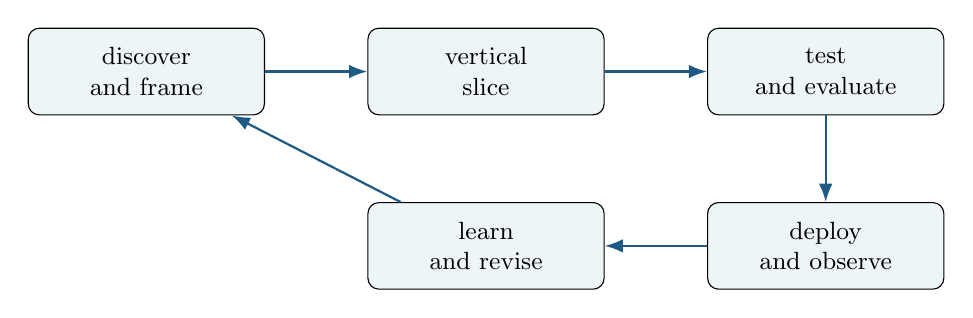
\begin{tikzpicture}[node distance=11mm and 13mm, every node/.style={font=\small}, box/.style={draw, rounded corners, fill=pale, minimum width=30mm, minimum height=11mm, align=center}, arr/.style={-{Latex}, thick, blue}]
\node[box] (discover) {discover\\and frame};
\node[box,right=of discover] (slice) {vertical\\slice};
\node[box,right=of slice] (evaluate) {test\\and evaluate};
\node[box,below=of evaluate] (operate) {deploy\\and observe};
\node[box,left=of operate] (learn) {learn\\and revise};
\draw[arr] (discover)--(slice);
\draw[arr] (slice)--(evaluate);
\draw[arr] (evaluate)--(operate);
\draw[arr] (operate)--(learn);
\draw[arr] (learn)--(discover);
\end{tikzpicture}
\caption{An incremental engineering loop that keeps discovery, delivery, and learning connected.}
\label{fig:engineering-loop}
\end{figure}

\section{Quality attributes and trade-offs}
A quality attribute becomes useful when it has a context, a measure, and a threshold. For CivicQueue:
\begin{itemize}
\item availability: the service is available during published booking hours;
\item confidentiality: citizens cannot view another person's case;
\item response time: the booking confirmation appears within a stated percentile under a stated load;
\item accessibility: core tasks can be completed with keyboard navigation and assistive technology;
\item maintainability: domain rules can be changed without editing presentation code.
\end{itemize}
These are not independent. Aggressive caching may improve speed but expose stale or private data. Strong verification may slow release but reduce risk. The team should document the trade-off rather than claim that all qualities are maximised.

\section{Version control, review, and integration}
Git records snapshots of a project and supports branching, comparison, and collaboration. A branch is a coordination mechanism, not a substitute for communication. A useful change has a small scope, a clear message, tests, and a review that examines behaviour and risk. Merging code is easy compared with integrating assumptions.

Continuous integration runs repeatable checks when changes are proposed. A minimal pipeline may format code, run unit tests, run integration tests, build the application, and produce an artefact. Continuous delivery adds a controlled path to deployment. Neither practice guarantees that a requirement is correct or that the system is usable.

\section{Technical debt and maintenance}
Technical debt is not simply bad code. It is a present choice that creates future cost, risk, or reduced option value. Some debt is deliberate and documented; some is accidental. A team should record why it exists, what interest it incurs, and when it should be repaid. Refactoring changes internal structure while preserving observable behaviour. It is safer when tests describe the behaviour that must remain stable.

\section{Professional responsibility}
A software engineer is accountable for communicating uncertainty and foreseeable harm. Security, privacy, accessibility, and inclusive design should appear in requirements and tests, not as a final polish step. A team should have an escalation path for unsafe requests, missing consent, data leakage, and conflicts between delivery pressure and professional standards.

\section{Project application}
A strong project report can include:
\begin{enumerate}
\item a problem formulation and stakeholder evidence;
\item a requirements table with source, priority, and acceptance criteria;
\item a decision log for architecture and scope;
\item a traceability matrix from requirement to test;
\item a delivery history showing iterations and feedback;
\item a quality and risk assessment;
\item a reflection on group work and technical debt.
\end{enumerate}
When presenting the work, do not turn the process into a success story. Explain a decision that was revised, an assumption that failed, and what evidence caused the change.

\section{Summary and key terms}
Software engineering coordinates people, models, code, tests, deployment, and maintenance under constraints. Requirements should be traceable and testable. Lifecycle models organise uncertainty but do not remove it. Quality attributes require context and trade-offs. Version control, review, integration, and technical-debt management are mechanisms for preserving reasoning across time.

\begin{keyterms}software engineering; requirement; acceptance criterion; traceability; lifecycle; incremental development; agile; quality attribute; reliability; technical debt; refactoring; version control; continuous integration; deployment.\end{keyterms}

\section{Exercises and worked solutions}
\exercise{Turn \enquote{the booking process should be user-friendly} into two testable requirements.}
\solution{One requirement could be that a first-time user can identify the rescheduling action from the appointment view without help in a defined usability test. Another could be that the rescheduling form can be completed using keyboard navigation and has a programmatically associated error message for each invalid field. The thresholds and study procedure must still be specified.}

\exercise{What is the difference between a feature and an acceptance criterion?}
\solution{A feature names a capability, such as rescheduling. An acceptance criterion states an observable condition under which a particular behaviour is considered acceptable, including relevant inputs, outputs, and failure handling.}

\exercise{Why is a small vertical slice useful before implementing the whole system?}
\solution{It exposes integration assumptions among interface, domain logic, persistence, and deployment. A broad component can look complete while the system cannot perform one user-visible task end to end.}

\section{Further reading}
Software development connects programming to requirements, demonstrable running systems, and explanations of how programs solve problems. Compare the Agile Manifesto with the Scrum Guide \citep{scrumguide2020}, and treat both as historical and practical sources rather than universal laws.

\chapter{Object-oriented and domain design}
\label{ch:oop}

\section{A motivating problem}
CivicQueue contains appointments, citizens, service types, slots, notifications, and staff actions. If the system stores everything as unrelated dictionaries, rules become scattered and inconsistent. If it creates a large hierarchy of classes, a small policy change can require changes across the entire program. Object-oriented design is a set of modelling and programming techniques for managing such complexity, not a command to turn every noun into a class.

\learningobjectives{You should be able to explain objects, identity, state, behaviour, encapsulation, interfaces, composition, inheritance, polymorphism, cohesion, coupling, dependency inversion, immutability, and testability; compare object-oriented design with procedural, functional, data-oriented, and component-based approaches; and refactor a domain model.}

\section{The five-minute explanation}
An object combines identity, state, and behaviour. A class is one way to define a family of objects. Encapsulation means that clients depend on a controlled interface rather than directly changing internal representation. An invariant is a condition the object promises to preserve.

For an appointment, the rule \enquote{a cancelled appointment cannot be completed} belongs close to the state it protects. This does not mean the object should contain database access, HTML rendering, and email delivery. Good design separates responsibilities while keeping domain rules explicit.

\section{A small domain model}
The following example uses Python dataclasses. It is intentionally incomplete; a production model would need time zones, identifiers, authorisation, persistence, and concurrency control.

\begin{lstlisting}[language=Python,caption={A domain object with an explicit state invariant.}]
from dataclasses import dataclass
from enum import Enum

class Status(Enum):
    REQUESTED = "requested"
    CONFIRMED = "confirmed"
    CANCELLED = "cancelled"
    COMPLETED = "completed"

@dataclass
class Appointment:
    identifier: int
    status: Status = Status.REQUESTED

    def confirm(self) -> None:
        if self.status is not Status.REQUESTED:
            raise ValueError("only requested appointments can be confirmed")
        self.status = Status.CONFIRMED

    def cancel(self) -> None:
        if self.status in {Status.CANCELLED, Status.COMPLETED}:
            raise ValueError("appointment cannot be cancelled")
        self.status = Status.CANCELLED

    def complete(self) -> None:
        if self.status is not Status.CONFIRMED:
            raise ValueError("only confirmed appointments can be completed")
        self.status = Status.COMPLETED
\end{lstlisting}

The methods define allowed transitions. The class does not know how the object is stored or displayed. This separation makes unit tests cheap and reduces coupling.

\section{Composition, inheritance, and polymorphism}
Composition builds an object from collaborating objects. Inheritance creates a subtype relation and can support substitutability, but it also couples subclasses to superclass decisions. Prefer composition when the relationship is \enquote{has a} or when behaviour should be selected at runtime. Use inheritance when a stable substitutable abstraction is genuinely present.

Polymorphism means that code can use a common interface while the concrete behaviour varies. In Python, protocols and duck typing can express this without a class hierarchy. A notification service might accept any object with a \texttt{send} method. The abstraction should be defined by the responsibility the caller needs, not by a taxonomy of vendors.

\section{SOLID principles as questions}
SOLID principles are heuristics, not proof rules:
\begin{description}
\item[Single responsibility] Which reason for change does this module own?
\item[Open--closed] Can a new variant be added without editing stable code?
\item[Liskov substitution] Does a subtype preserve the promises clients rely on?
\item[Interface segregation] Are clients forced to depend on operations they do not use?
\item[Dependency inversion] Does high-level policy depend on abstractions rather than infrastructure details?
\end{description}
Applying a principle mechanically can produce needless indirection. A small program may be clearer with a function than with five interfaces.

\section{Cohesion, coupling, and immutability}
Cohesion asks whether the responsibilities in a module belong together. Coupling asks how much one module knows about another. Immutability reduces the number of possible state histories. A value object such as a \texttt{SlotId} or a date range can be immutable and validated at construction. Mutable aggregate objects require stronger invariants and careful ownership.

\section{Patterns and their forces}
A design pattern describes a recurring problem, the forces that shape it, a structure, and consequences. The Repository pattern can separate domain code from persistence; Dependency Injection can make infrastructure replaceable in tests; Adapter can translate an external API; Strategy can select an algorithm; Observer can notify dependants about an event. MVC separates concerns in interactive applications, but the boundaries depend on the framework and can become confused.

The common misuse is pattern naming without problem analysis. Ask what change or force the pattern addresses, what complexity it introduces, and whether a simpler function or module would be better. The original catalogue remains useful as a language for design discussion \citep{gamma1994design}.

\section{Alternatives to object orientation}
Procedural decomposition can be clearer for transformations. Functional programming emphasises pure functions and immutable data. Data-oriented design organises around memory layout and operations over data. Component-based design composes independently deployable or replaceable parts. A realistic system often combines all four. The criterion is clarity of invariants and change boundaries, not ideological consistency.

\section{Testing and refactoring}
Test domain objects through public behaviour. Test an invariant's boundary cases, not just the happy path. Refactor after a test suite gives a safety net. If a class requires a database, clock, network, and global configuration to construct, the design is telling you that responsibilities are mixed or dependencies are hidden.

\section{Project application}
When documenting the work, include a domain model and explain which concepts are entities, value objects, services, or external systems. Show one design alternative you rejected and the force that made it less suitable. When presenting it, explain why a domain rule lives where it does and how the design would change if a second notification channel were added.

\section{Summary and key terms}
Objects protect state and expose behaviour through interfaces. Composition is often safer than inheritance for reuse. Polymorphism supports substitutable variation. SOLID principles are questions about change, substitution, and dependency, not automatic templates. Patterns are named responses to forces. Procedural, functional, data-oriented, and component-based designs remain legitimate alternatives.

\begin{keyterms}object; identity; state; behaviour; class; instance; encapsulation; abstraction; interface; composition; inheritance; polymorphism; dynamic dispatch; cohesion; coupling; immutability; dependency inversion; design pattern.\end{keyterms}

\section{Exercises and worked solutions}
\exercise{Why should an appointment object reject an invalid transition rather than let any caller assign its status?}
\solution{If callers can assign arbitrary status values, the invariant is distributed across every caller and can be violated by omission. A method or validated state transition centralises the rule. The object still needs integration tests and authorisation at a higher level; encapsulation does not solve every concern.}

\exercise{Give one reason to prefer composition over inheritance for notifications.}
\solution{A service may need to send through email, SMS, or a queue depending on configuration. Composing an appointment service with a notification interface allows the strategy to change without making \texttt{EmailNotification} and \texttt{SmsNotification} subclasses of an artificial common object.}

\exercise{When can a design pattern make a project worse?}
\solution{It can add indirection, obscure a simple control flow, create more classes to maintain, or imply a fixed structure when the forces are not present. The pattern should earn its complexity by addressing a real change or coordination problem.}

\section{Further reading}
Use access, encapsulation, resource management, and security as questions for analysing a design. Compare the patterns catalogue \citep{gamma1994design} with the enterprise patterns in \citet{fowler2002patterns}.

\chapter{Systems analysis and modelling}
\label{ch:modelling}

\section{A motivating problem}
A team says that CivicQueue needs \enquote{a calendar integration}. One person imagines a public booking calendar; another imagines a staff scheduling service; a third imagines a synchronisation job. The sentence is too compressed to coordinate design. A model externalises the assumptions so that people can inspect, question, and revise them.

\learningobjectives{You should be able to use models to analyse and communicate systems; define boundaries, actors, responsibilities, events, interfaces, and contracts; choose appropriate UML diagrams; explain design patterns as responses to forces; and assess model--code consistency.}

\section{The five-minute explanation}
A model is a selective representation made for a purpose. A use-case model helps discuss goals and actors. A class model describes concepts and relationships. A sequence model describes an interaction over time. A state machine describes legal transitions. A component model describes replaceable units and dependencies. No diagram is the system itself.

\plainlanguage{A diagram is valuable when it lets a team notice, remember, or negotiate something that would otherwise remain hidden. It is harmful when its symbols create a false sense of precision.}

\section{Problem and application domains}
The problem domain contains the situation the system is meant to address: appointments, citizens, staff work, and rules. The application domain contains the technical artefact and its interfaces. A good model relates the two without assuming that a software class is identical to a real-world institution.

Define the system boundary before drawing. List actors by the goals they pursue, not merely by the screens they use. An external identity provider may be an actor in a system interaction even when no human directly sees it.

\section{Use cases and requirements}
A use case describes a goal-oriented interaction. \enquote{Reschedule appointment} is a goal; \enquote{click button} is an interaction step. A use-case narrative should include preconditions, trigger, main success scenario, alternatives, failure conditions, and postconditions.

\begin{figure}[H]
\centering
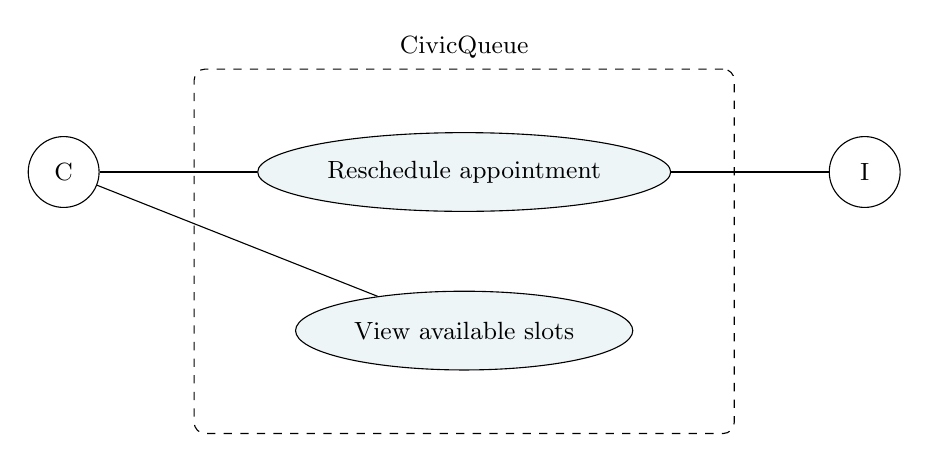
\begin{tikzpicture}[node distance=10mm and 20mm, every node/.style={font=\small}, actor/.style={draw, circle, minimum size=9mm}, use/.style={draw, ellipse, fill=pale, minimum width=36mm, minimum height=10mm}, boundary/.style={draw, rounded corners, dashed, inner sep=8mm}]
\node[actor] (citizen) {C};
\node[use,right=of citizen] (reschedule) {Reschedule appointment};
\node[use,below=of reschedule] (view) {View available slots};
\node[actor,right=of reschedule] (identity) {I};
\node[boundary,fit=(reschedule)(view),label=above:CivicQueue] (system) {};
\draw (citizen)--(reschedule);
\draw (citizen)--(view);
\draw (identity)--(reschedule);
\end{tikzpicture}
\caption{A use-case boundary with a citizen actor and an external identity service.}
\label{fig:usecase}
\end{figure}

The abbreviations C and I are explained in the caption or surrounding text. Avoid relying on a visual legend alone.

\section{Class and domain models}
A class diagram can show entities, value objects, associations, multiplicities, and responsibilities. It should distinguish an appointment from an appointment slot: one is a booked occurrence; the other is an available capacity at a time and service location. If a rescheduling operation creates a new appointment, the model should make that identity decision visible.

A domain model is not a database schema. It may contain concepts that are derived, transient, or intentionally absent from persistence. Conversely, a database may contain technical fields such as audit timestamps and indexes that do not belong in the domain vocabulary.

\section{Behavioural models}
A sequence diagram shows messages between participants:
\begin{enumerate}
\item the citizen submits a rescheduling request;
\item the interface sends an HTTP request;
\item the application authorises the action;
\item the domain service checks the state transition;
\item the repository performs a transaction;
\item the response reports success or a conflict;
\item the interface gives feedback.
\end{enumerate}
A state machine models legal histories. An activity diagram models control and responsibility. Use the smallest model that answers the question being asked.

\section{Contracts}
A contract specifies an interface's preconditions, postconditions, and invariants. For a slot-reservation operation:
\begin{itemize}
\item precondition: the caller is authorised and the slot is available;
\item postcondition on success: exactly one reservation owns the slot;
\item postcondition on conflict: the slot ownership is unchanged;
\item invariant: one slot cannot have two active reservations.
\end{itemize}
Contracts expose concurrency requirements that a class diagram alone may hide.

\section{Architecture and patterns}
At a high level, CivicQueue can be separated into presentation, application services, domain logic, persistence, and external adapters. MVC can help organise a web interface. Repository hides persistence details. Adapter isolates a calendar provider. Dependency Injection makes the application service testable. Observer may model notifications, but asynchronous delivery introduces retries and duplicate-event concerns.

Patterns are not decorations. For each pattern, state the problem, forces, structure, consequences, alternatives, and misuse. A repository is not automatically better than a direct query; it is useful when the persistence boundary is meaningful and stable.

\section{Model--code consistency}
Models decay when code changes without updating them, but freezing every diagram can slow development. Keep diagrams that support decisions, onboarding, safety, or communication. Link them to code modules and tests. Delete a diagram when it no longer represents a decision that anyone uses.

\section{Project application}
Choose one diagram per question. Include a system boundary early, a domain model before implementation, and a sequence or state model for the most failure-prone interaction. When documenting the work, explain abstraction choices and inconsistencies. When presenting it, be prepared to redraw the model when someone changes an actor, permission, or failure condition.

\section{Summary and key terms}
Modelling is a way of thinking and coordinating, not diagram production. Different diagrams answer different questions. Boundaries, actors, responsibilities, events, interfaces, contracts, and invariants connect problem analysis to implementation. Patterns are justified by forces and consequences. Models should be maintained selectively and honestly.

\begin{keyterms}model; system boundary; actor; use case; domain model; UML; class diagram; sequence diagram; state machine; activity; component; deployment; interface; contract; precondition; postcondition; design pattern; architecture.\end{keyterms}

\section{Exercises and worked solutions}
\exercise{Why is \enquote{calendar integration} a poor requirement? Rewrite it as a use-case goal and one acceptance criterion.}
\solution{It names a technical solution without a user goal or boundary. A goal is \enquote{a staff member can publish available appointment slots from the authoritative schedule}. An acceptance criterion could state that a published slot is shown with the correct service, time zone, and availability, and that a failed synchronisation leaves the previous published state visible with an error recorded.}

\exercise{Which diagram is most useful for showing that a cancelled appointment cannot be completed?}
\solution{A state-machine diagram directly represents legal transitions. A class diagram may show a status attribute, and a sequence diagram may show one scenario, but neither alone states all allowed histories as clearly.}

\exercise{What makes a diagram misleading?}
\solution{Ambiguous names, hidden boundaries, missing failure paths, inconsistent notation, false precision, and an outdated relationship to code can all mislead. A diagram should state its purpose and scope.}

\section{Further reading}
The UML specification provides a standard notation \citep{omg2017uml}. This book treats modelling as a means of reasoning rather than a compliance exercise.

\chapter{Web and full-stack application development}
\label{ch:web}

\section{A motivating problem}
A citizen clicks \enquote{request new time}. The browser sends a request through a network. The server authenticates the user, checks authorisation, validates the input, applies a domain rule, writes data, and returns a response. The browser renders feedback. If any step is misunderstood, the prototype may work only on the developer's machine.

\learningobjectives{You should be able to trace a request through a full-stack system; explain HTTP, REST-style resource design, JSON, client and server responsibilities, authentication and authorisation; design validation and error handling; and discuss configuration, deployment, monitoring, and architectural trade-offs.}

\section{The five-minute explanation}
A full-stack application is a set of cooperating layers:
\begin{enumerate}
\item the client presents information and captures interaction;
\item the network transports a request and response;
\item the server applies application and domain logic;
\item persistence stores and retrieves durable state;
\item external services provide identity, notifications, or other capabilities;
\item operation practices keep the system observable and changeable.
\end{enumerate}
The layers are not physical boxes in every deployment. They are responsibilities that should be identifiable.

\begin{figure}[H]
\centering
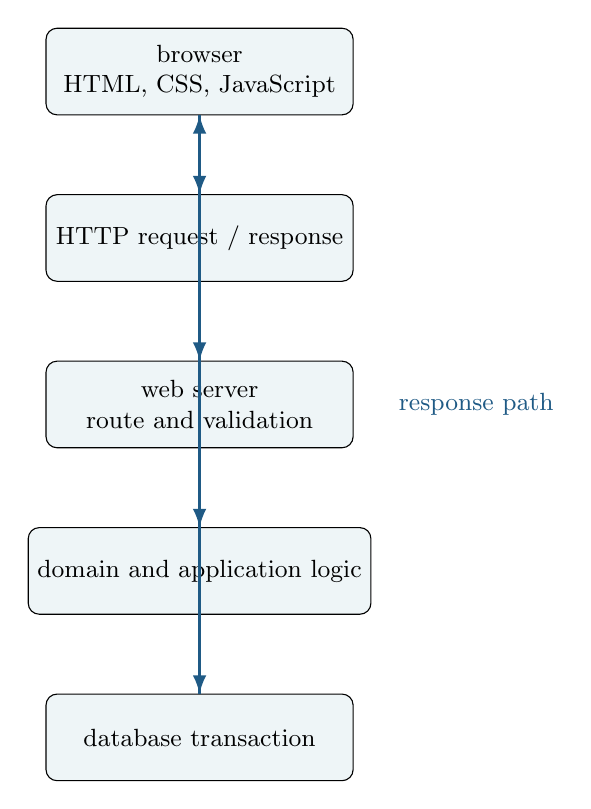
\begin{tikzpicture}[node distance=10mm, every node/.style={font=\small}, box/.style={draw, rounded corners, fill=pale, minimum width=39mm, minimum height=11mm, align=center}, arr/.style={-{Latex}, thick, blue}]
\node[box] (browser) {browser\\HTML, CSS, JavaScript};
\node[box,below=of browser] (http) {HTTP request / response};
\node[box,below=of http] (server) {web server\\route and validation};
\node[box,below=of server] (domain) {domain and application logic};
\node[box,below=of domain] (db) {database transaction};
\draw[arr] (browser)--(http);
\draw[arr] (http)--(server);
\draw[arr] (server)--(domain);
\draw[arr] (domain)--(db);
\draw[arr] (db)--node[right,xshift=24mm]{response path}(browser);
\end{tikzpicture}
\caption{The path of a CivicQueue request. Every arrow is a possible failure boundary.}
\label{fig:request-path}
\end{figure}

\section{HTTP and resource design}
HTTP has methods, status codes, headers, and a message body. A \texttt{GET} should retrieve a representation without changing server state; a \texttt{POST} commonly requests creation or an action; \texttt{PUT} replaces a resource representation; \texttt{PATCH} partially modifies it; \texttt{DELETE} requests removal. These are conventions with semantics, not magic names.

A REST-style API exposes resources and representations. For CivicQueue, a client might request \texttt{GET /api/appointments/42} or \texttt{POST /api/appointments/42/reschedule}. The second path is an action endpoint; a different design could model a rescheduling request as a new resource. The choice should reflect domain meaning and idempotency.

\section{Frontend state and feedback}
The browser has state: the current route, form values, loading status, errors, and cached data. Do not show success before the server confirms success. Disable or de-duplicate a submission only when the interaction design and server semantics support it. Accessible feedback must be perceivable by people who do not see a visual colour change.

\section{Backend boundaries}
A route should translate an HTTP request into an application call and an application result into an HTTP response. It should not contain every domain rule and SQL query. A small Flask route can look like this:

\begin{lstlisting}[language=Python,caption={A deliberately thin route boundary.}]
@app.post("/api/appointments/<int:appointment_id>/cancel")
def cancel_appointment(appointment_id: int):
    actor = current_user()
    result = appointment_service.cancel(appointment_id, actor)
    if result.is_not_found:
        return {"error": "appointment not found"}, 404
    if result.is_forbidden:
        return {"error": "not allowed"}, 403
    if result.is_conflict:
        return {"error": "appointment cannot be cancelled"}, 409
    return {"status": "cancelled"}, 200
\end{lstlisting}

The service contains the policy; the repository handles persistence; the route maps outcomes to protocol responses. Error messages should not disclose information to unauthorised callers.

\section{Authentication and authorisation}
Authentication answers who the actor is. Authorisation answers what that actor may do. A valid login does not grant access to every appointment. Enforce authorisation on the server for every protected operation. Sessions usually store a server-side identifier in a secure cookie; tokens can carry claims but require careful expiry, storage, rotation, and revocation decisions. Do not put secrets in browser code.

\section{Validation and error handling}
Validate at multiple boundaries. Client-side validation improves feedback; server-side validation is authoritative. Validate type, range, format, ownership, state, and business rules. Use status codes consistently: malformed input may be 400, unauthenticated 401, forbidden 403, missing 404, conflict 409, and unexpected failure 500. Do not expose stack traces in production.

\section{Configuration, migrations, and deployment}
Configuration varies across environments and should be supplied through environment variables or a managed configuration system. Secrets should not be committed to Git. Database schema changes need migrations that can be reviewed, applied, and rolled back or forward safely. A container packages an application and its runtime assumptions, but it does not automatically make the system secure or scalable.

A small deployment needs a process manager, TLS termination, database backups, logs, health checks, and a rollback plan. Twelve-factor principles are useful reminders about configuration, stateless processes, logs, and disposability, but they must be adapted to the system's data and operational context.

\section{Performance and scalability}
Measure the path that users experience. Network latency, database indexes, serialisation, queueing, and rendering all contribute. Horizontal scaling creates coordination questions about sessions, caches, transactions, and background jobs. Microservices are not a maturity badge; they add network boundaries, deployment complexity, and distributed failure modes. A modular monolith can be a better starting point.

\section{The recurring case implementation}
The supplied example application uses Flask and SQLite to remain small enough to inspect. It includes:
\begin{itemize}
\item an HTML interface and JSON endpoints;
\item a domain service for appointment state;
\item parameterised SQL;
\item database initialisation and seed data;
\item tests for domain and request behaviour;
\item a clear limitation: authentication is a demonstration boundary, not production identity.
\end{itemize}
Read the directory before changing it. Trace one request from browser form to response, then add one failure test.

\section{Project application}
Show the request lifecycle in a diagram, document API contracts, and explain where authentication, authorisation, validation, persistence, and error mapping occur. When presenting the work, be prepared to answer what happens when the request is repeated, the database is unavailable, the external service times out, or the browser submits stale data.

\section{Summary and key terms}
Full-stack development connects client interaction, HTTP, server logic, domain rules, persistence, and operation. Protocol semantics and domain semantics should not be confused. Authentication and authorisation are different. Validation belongs at trust boundaries. Deployment requires configuration, migrations, observability, security, and recovery plans.

\begin{keyterms}client; server; HTTP; REST; resource; JSON; frontend state; backend; domain logic; persistence; authentication; authorisation; session; token; validation; migration; container; deployment; observability; scalability.\end{keyterms}

\section{Exercises and worked solutions}
\exercise{Why is returning HTTP 200 before the database transaction commits dangerous?}
\solution{The client receives a success claim before the durable state is known to exist. A later failure can leave the user and system with different beliefs. The response should reflect the transaction result or explicitly represent an asynchronous pending state.}

\exercise{A user can view their own appointment but changes the URL to another identifier. Which security property is missing?}
\solution{Server-side object-level authorisation is missing. Authentication identifies the caller but does not establish that the caller may access the referenced appointment. The service must check ownership or another explicit permission.}

\exercise{When is a modular monolith preferable to microservices?}
\solution{When the domain and team boundaries are still uncertain, deployment scale is modest, and a single transaction or shared model simplifies correctness. Services can be extracted later when the boundary and operational benefit justify the distributed-system cost.}

\section{Further reading}
HTTP semantics are specified in RFC 9110 \citep{rfc9110}; REST is an architectural style described in \citet{fielding2000architectural}. Use the HTML standard \citep{whatwghtml} and the OWASP guidance \citep{owasptop10} for implementation and security details.

\chapter{Databases and durable information}
\label{ch:databases}

\section{A motivating problem}
A spreadsheet can record appointments until several people edit it at once. Then duplicates appear, a citizen's status disagrees with the staff calendar, and nobody can explain which value is authoritative. A database is not merely a faster spreadsheet. It is a system for representing, constraining, querying, and updating shared state.

\learningobjectives{You should be able to explain the relational model; design entities, keys, and integrity constraints; use SQL selection, projection, joins, aggregation, subqueries, and views; reason about functional dependencies and normal forms; explain transactions, isolation, locks, indexes, migrations, and database security; and compare relational and non-relational models.}

\section{The five-minute explanation}
A relation is a set of tuples with attributes. In a table, rows represent tuples and columns represent attributes, but a relational relation is not defined by its visual layout. A key identifies a tuple. A foreign key expresses a relationship between tables. Constraints prevent states that the domain says are invalid.

Codd's relational model separated logical data relationships from physical storage decisions \citep{codd1970relational}. SQL is a declarative language: the query states what result is wanted, while the database chooses an execution plan.

\section{From domain concepts to schema}
The CivicQueue schema distinguishes:
\begin{itemize}
\item \texttt{citizens}, identified by a surrogate identifier and containing minimal contact data;
\item \texttt{services}, such as benefits advice or permit support;
\item \texttt{slots}, which represent available service capacity;
\item \texttt{appointments}, which connect one citizen to one slot;
\item \texttt{audit\_events}, which record security-relevant changes.
\end{itemize}
The schema in \texttt{examples/sql/schema.sql} can be loaded into SQLite. It uses primary keys, foreign keys, a uniqueness constraint, and a check constraint. Constraints are executable domain claims.

\section{Relational operations and SQL}
Selection filters rows; projection chooses attributes; a join combines related tuples. SQL expresses these operations:

\begin{lstlisting}[language=SQL,caption={A query that joins appointments to citizens and services.}]
SELECT a.id,
       c.display_name,
       s.name AS service_name,
       sl.starts_at,
       a.status
FROM appointments AS a
JOIN citizens AS c ON c.id = a.citizen_id
JOIN slots AS sl ON sl.id = a.slot_id
JOIN services AS s ON s.id = sl.service_id
WHERE a.status = 'confirmed'
ORDER BY sl.starts_at;
\end{lstlisting}

The query names the relationship conditions. An implicit join or a \texttt{SELECT *} can be shorter but may hide assumptions and create unstable interfaces. Use aliases and select the fields the client actually needs.

Aggregation uses functions such as \texttt{COUNT}, \texttt{AVG}, and \texttt{SUM}. \texttt{GROUP BY} changes the unit of analysis. If you count appointments by service, the result is no longer one row per appointment; it is one row per service. State that change explicitly.

\section{Functional dependencies and normalisation}
A functional dependency $X\rightarrow Y$ means that equal values of attributes $X$ require equal values of attributes $Y$ in the relation. If \texttt{service\_id} determines \texttt{service\_name}, storing both repeatedly in an appointment table creates update anomalies:
\begin{itemize}
\item update anomaly: renaming a service requires many edits;
\item insertion anomaly: a service cannot be stored without an appointment;
\item deletion anomaly: deleting the last appointment removes the service description.
\end{itemize}
Normalisation decomposes relations to reduce such anomalies while preserving dependencies and joinability. First, second, third normal form, and BCNF are conditions with different strengths. They are not a ritual of splitting every table. Denormalisation can be justified for measured read performance, reporting, or integration, but its duplicated facts need a consistency strategy.

\section{Transactions and ACID}
A transaction groups operations so that the database enforces a defined unit of change. ACID abbreviates atomicity, consistency, isolation, and durability. The terms do not mean that every transaction is globally correct: consistency depends on constraints and application rules; isolation has levels and trade-offs.

For rescheduling, one transaction may check the new slot, insert a new appointment, cancel or release the old slot, and write an audit event. If any required step fails, the transaction should roll back. Two concurrent transactions can still conflict unless the database and application use an appropriate constraint or locking strategy.

\section{Isolation and concurrency}
At lower isolation, transactions may see phenomena such as dirty reads, non-repeatable reads, or phantoms. At higher isolation, the database may block or abort more work. A unique constraint on an active slot can be safer than a check-then-insert sequence because the database arbitrates the race. Retry logic must distinguish transient serialization failures from permanent validation errors.

\section{Indexes and query plans}
An index is an auxiliary structure that can reduce search work at the cost of storage and write overhead. Index columns used in filters, joins, and ordering when measurement supports it. An index on a low-selectivity column may offer little benefit. Inspect query plans and benchmark representative data. Indexes do not fix an incorrect query or a missing authorisation condition.

\section{Migrations, backups, and security}
A migration changes schema in a controlled, versioned step. Backups should be encrypted, tested by restoration, and governed by retention rules. Use parameterised queries; never concatenate user input into SQL. Limit database credentials by environment and privilege. Logs can themselves contain personal data and require access control and retention decisions.

\section{NoSQL and polyglot persistence}
Document stores, key-value stores, graph databases, and wide-column systems optimise different access patterns and consistency models. A document model can be convenient for nested data, a graph model for relationship traversal, and a key-value store for predictable lookups. The choice should follow data shape, query patterns, consistency, transaction scope, operations, and team capability. \enquote{NoSQL} is not one model and does not automatically scale better.

\section{Project application}
Include an ER or relational design, functional dependencies, constraints, representative queries, transaction boundaries, indexes with evidence, migration strategy, and security analysis. When presenting the work, explain what anomaly the normalisation choice prevents and what trade-off a denormalised read model would introduce.

\section{Summary and key terms}
Databases make shared state durable and constrain its structure. The relational model supports declarative queries and integrity constraints. Normalisation is about dependencies and anomalies. Transactions coordinate changes; isolation manages concurrency trade-offs. Indexes, migrations, backups, parameterised queries, and access control are engineering parts of data management.

\begin{keyterms}relation; tuple; attribute; key; foreign key; constraint; join; aggregation; functional dependency; normalisation; denormalisation; transaction; ACID; isolation; lock; index; query plan; migration; backup; NoSQL.\end{keyterms}

\section{Exercises and worked solutions}
\exercise{Why is a citizen's display name usually not a fact that should be copied into every appointment row?}
\solution{The citizen identifier determines the current identity record, while repeated display names can become inconsistent after a correction. A report may intentionally snapshot a historical name, but then the snapshot is a different documented fact with a retention and audit rationale.}

\exercise{What can go wrong with a check-then-insert reservation sequence?}
\solution{Two concurrent transactions can both observe the slot as available and then both insert. A database uniqueness constraint, appropriate transaction isolation, or an atomic reservation operation is needed to make the invariant hold under concurrency.}

\exercise{When can denormalisation be justified?}
\solution{When a measured access pattern needs faster reads or simpler analytical queries, and the duplication has an explicit update, reconciliation, and testing strategy. It should be a response to a stated constraint, not an assumption that joins are always bad.}

\section{Further reading}
For foundations, read \citet{garciamolina2008database} and \citet{date2003introduction}. PostgreSQL's documentation is a practical reference for a production relational system \citep{postgresdocs}; the example project uses SQLite to keep setup small.

\chapter{Security, testing, and operations}
\label{ch:operations}

\section{A motivating problem}
A prototype can pass its demo while exposing appointments through predictable URLs, logging personal data, accepting forged requests, and failing silently when an email provider is unavailable. Security and operations are not separate from development; they describe what the system must preserve in an adversarial and changing environment.

\learningobjectives{You should be able to threat-model an application; distinguish authentication, authorisation, confidentiality, integrity, and availability; recognise common web vulnerabilities; design layered tests and CI checks; and explain logging, metrics, tracing, deployment, incident response, and recovery.}

\section{The five-minute explanation}
Security is the reduction of unacceptable risk to assets under threats and constraints. A threat model identifies assets, actors, trust boundaries, possible abuse paths, and mitigations. It is not a promise that no attack can succeed. Operations asks whether the system can be observed, changed, recovered, and governed after deployment.

\section{Threat modelling CivicQueue}
Assets include appointment confidentiality, slot integrity, citizen contact data, staff accounts, audit records, and service availability. Threats include account takeover, insecure direct object references, SQL injection, cross-site scripting, cross-site request forgery, malicious file input, notification abuse, and denial of service. Draw trust boundaries between browser, application, database, identity provider, and notification service.

For each risk, record:
\begin{enumerate}
\item asset and harm;
\item attacker capability and precondition;
\item likelihood and impact rationale;
\item preventive and detective controls;
\item residual risk and owner.
\end{enumerate}
OWASP's Top 10 provides a vocabulary for common application risks, while NIST's Secure Software Development Framework connects security practices to the development lifecycle \citep{owasptop10,nistssdf}.

\section{Secure defaults}
Use parameterised SQL, output encoding, server-side authorisation, secure cookie attributes, CSRF protection for state-changing browser requests, password hashing through a vetted library, TLS, rate limits, dependency updates, and least-privilege credentials. Do not invent cryptography. Do not log passwords, access tokens, or unnecessary personal data. Return generic errors to untrusted callers while preserving useful internal diagnostics.

Security controls can create usability costs. A short session timeout may reduce risk but create barriers for users with cognitive or motor impairments. The trade-off should be evaluated and supported by recovery paths.

\section{Testing as layered evidence}
A testing strategy has layers:
\begin{description}
\item[Unit] Does one function or domain object satisfy its contract?
\item[Integration] Do components interact correctly with a real or controlled database and external boundary?
\item[System] Does the deployed application perform a complete user task?
\item[Property and invariant] Does a rule hold across generated inputs?
\item[Security] Can an unauthorised actor violate confidentiality or integrity?
\item[Usability and accessibility] Can intended users complete tasks and recover from errors?
\end{description}
A high percentage of unit coverage does not imply high system quality. Tests should be selected from risks and requirements, not from a desire to maximise a single number.

\section{Continuous integration and delivery}
A CI pipeline should fail clearly and reproducibly. Typical steps are dependency installation from a lock or constrained file, linting, type checks, unit tests, integration tests, security checks, packaging, and build verification. A deployment pipeline promotes an immutable artefact through environments with approvals appropriate to risk. Database migrations and rollback plans belong in the release design.

\section{Observability and reliability}
Logs record events; metrics aggregate measurements; traces follow a request across components. Use correlation identifiers rather than personal identifiers where possible. Define service-level indicators such as successful booking rate and latency. An alert should have an owner and an action, not merely report that a graph changed.

Reliability includes failure handling: timeouts, retries with backoff, idempotency keys, circuit breakers, graceful degradation, backup restoration, and incident review. Retrying a non-idempotent reservation can create duplicates. Make the operation's semantics explicit.

\section{Performance and capacity}
Capacity planning estimates demand and resource limits. A queue, database connection pool, and notification provider can each become the bottleneck. Load tests should use representative traffic and safe data. Report uncertainty and environmental limits. Do not interpret a local benchmark as a guarantee about production.

\section{Accessibility and privacy in operation}
Accessibility is not finished at the interface layer if an outage removes the only accessible route. Privacy includes logs, backups, analytics, monitoring, support access, and data deletion. Data retention should be justified by purpose and legal context. A system that is secure from attackers but unusable by the intended population has failed a central requirement.

\section{Project application}
Include a threat model, test strategy, CI evidence, deployment diagram, operational assumptions, and recovery scenario. Demonstrate one failure intentionally: disconnect the database, submit an invalid transition, or replay a request. When documenting the work, distinguish a vulnerability you mitigated from a risk you merely documented.

\section{Summary and key terms}
Security and operations extend engineering beyond the happy path. Threat modelling connects assets to risks and controls. Authentication is not authorisation. Layered tests provide different evidence. Observability, reliability, deployment, backup, and recovery are design concerns. Privacy and accessibility continue through logs and operations.

\begin{keyterms}threat model; asset; trust boundary; authentication; authorisation; confidentiality; integrity; availability; SQL injection; XSS; CSRF; least privilege; unit test; integration test; CI/CD; observability; log; metric; trace; idempotency; incident response.\end{keyterms}

\section{Exercises and worked solutions}
\exercise{A request to cancel an appointment is retried after a timeout. What should the design consider?}
\solution{The server may have completed the first request even though the client did not receive the response. The operation should be idempotent or use an idempotency key so that a retry does not create a second effect. The response should represent the current state consistently.}

\exercise{Why is \enquote{we use HTTPS} not a complete security argument?}
\solution{HTTPS protects transport under its assumptions, but it does not prevent broken authorisation, injection, insecure cookies, weak passwords, malicious application logic, leaked secrets, or harmful logging. Security is a set of controls across the system.}

\exercise{Give one example of an operational metric that is not merely server CPU.}
\solution{The proportion of successful booking attempts, the p95 confirmation latency, notification delivery failure rate, or the number of unauthorised access attempts may be more directly connected to user and security outcomes than CPU alone.}

\section{Further reading}
Use OWASP's Top 10 and Application Security Verification Standard as practical starting points \citep{owasptop10}; use NIST SP 800-218 for secure development practices \citep{nistssdf}. Reliability concepts should be connected to the system's actual failure modes rather than copied as a checklist.


\part{People, organisations, and development practice}
\chapter{Interaction design and human--computer interaction}
\label{ch:hci}

\section{A motivating problem}
A CivicQueue prototype contains every required field and still confuses users. Citizens do not know whether a slot is reserved, staff cannot tell which changes need approval, and an error message says only \enquote{invalid input}. The problem is not visual taste. It is the relationship between a person, a goal, a representation, an action, and feedback.

\learningobjectives{You should be able to explain perception, attention, memory, mental models, affordances, signifiers, feedback, constraints, mapping, cognitive load, errors and recovery, user-centred design, participatory methods, information architecture, interaction flows, and accessibility; and distinguish a design preference from an empirical claim.}

\section{The five-minute explanation}
Interaction design shapes what people can do, what they think they can do, and what the system communicates about what happened. A good interface does not eliminate human judgment; it supports people in forming an accurate working understanding and recovering when things go wrong.

\plainlanguage{If a button looks available, users may expect it to work. If a change is saved but no feedback appears, users may repeat the action. If the only error message is red text, a person who cannot see colour may miss it. Design is the management of expectations and consequences.}

\section{Human cognition and action}
People have limited attention and working memory. They use recognition, prior knowledge, external cues, and routines. A mental model is the user's working explanation of how a system behaves. Interfaces can support or disrupt that model. The goal is not to memorise a fixed number of interface rules; it is to reduce unnecessary cognitive work while making important distinctions visible.

Affordance describes what an object allows; a signifier communicates how it may be used. A flat rectangle may afford clicking in software but needs a signifier such as label, focus style, and pointer behaviour. Feedback tells the user what happened. Constraints prevent invalid actions or make them harder. Mapping connects controls to effects. These concepts are related but not interchangeable.

\section{User-centred and participatory design}
User-centred design is an iterative process involving users, tasks, context, prototyping, and evaluation. Participatory design gives affected people a role in shaping the problem and solution, not only in testing a finished interface. Neither approach guarantees fairness: the recruited users may not represent people with less power, and organisational constraints may limit which suggestions can be adopted.

Useful methods include:
\begin{description}
\item[Contextual inquiry] Observe work in context while asking about actions and exceptions.
\item[Interview] Elicit experiences, goals, language, and interpretations; do not treat reported preference as direct evidence of behaviour.
\item[Observation] Record what happens, including workarounds, interruptions, and artefacts.
\item[Task analysis] Decompose a goal into actions, decisions, information needs, and failure recovery.
\item[Persona] A synthesis of research patterns, not a fictional stereotype.
\item[Scenario] A situated narrative that makes goals, context, and constraints concrete.
\end{description}

\section{Information architecture and interaction flows}
Information architecture organises content and actions so that users can find, interpret, and navigate them. For CivicQueue, \enquote{My appointments}, \enquote{Available services}, and \enquote{Help and alternatives} may be more understandable than internal database categories. An interaction flow should include the start state, action, system feedback, alternative paths, error recovery, and end state.

\begin{figure}[H]
\centering
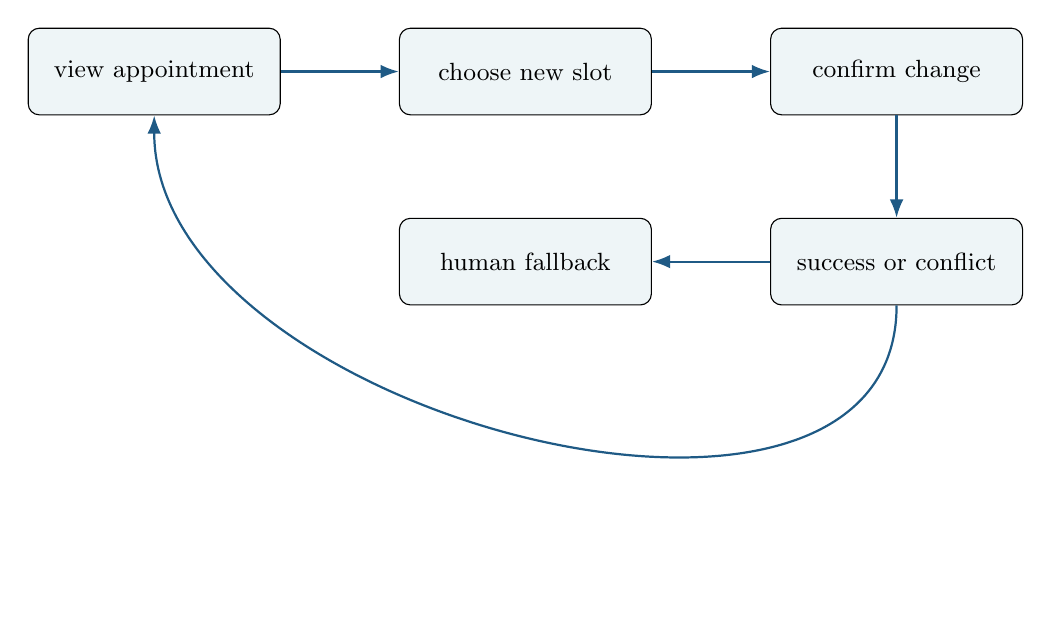
\begin{tikzpicture}[node distance=13mm and 15mm, every node/.style={font=\small}, box/.style={draw, rounded corners, fill=pale, minimum width=32mm, minimum height=11mm, align=center}, arr/.style={-{Latex}, thick, blue}]
\node[box] (view) {view appointment};
\node[box,right=of view] (choose) {choose new slot};
\node[box,right=of choose] (confirm) {confirm change};
\node[box,below=of confirm] (feedback) {success or conflict};
\node[box,left=of feedback] (help) {human fallback};
\draw[arr] (view)--(choose);
\draw[arr] (choose)--(confirm);
\draw[arr] (confirm)--(feedback);
\draw[arr] (feedback)--(help);
\draw[arr] (feedback.south) to[out=270,in=270] (view.south);
\end{tikzpicture}
\caption{An interaction flow includes success, conflict, and recovery paths.}
\label{fig:interaction-flow}
\end{figure}

\section{Prototyping}
A paper sketch, wireframe, clickable prototype, and working system answer different questions. Low-fidelity prototypes make information architecture and task flow cheap to change. High-fidelity prototypes can test visual hierarchy and interaction timing but may cause stakeholders to infer that backend behaviour already exists. Label what is real, simulated, or intentionally omitted.

\section{Visual hierarchy and inclusive design}
Typography, spacing, grouping, contrast, and alignment communicate structure. Aesthetic consistency can support recognition, but preference is not usability evidence. Accessibility includes semantic structure, keyboard operation, focus visibility, contrast, text resizing, captions, error identification, and compatibility with assistive technology. WCAG 2.2 provides testable success criteria, but conformance alone does not prove that a particular service is usable in context \citep{w3cwcag22}.

Inclusive design asks who is absent from the default. Consider language, literacy, motor and sensory variation, cognitive load, device access, connectivity, age, and institutional trust. A digital-only process may be efficient for one group and exclusionary for another.

\section{Ethics, privacy, and dark patterns}
An interface can manipulate through hidden costs, confusing consent, forced continuity, or defaults that benefit the provider over the user. Dark-pattern analysis asks who gains from the friction and who bears it. Privacy-friendly design uses data minimisation, clear purposes, granular choices, and deletion or correction routes. A consent checkbox cannot repair an interface that makes refusal practically impossible.

\section{Project application}
Ground design decisions in observed tasks and stakeholder language. Include a rationale for the interaction structure, a prototype history, accessibility considerations, and a map from problem to design response. When presenting the work, distinguish what users said, what they did, what you inferred, and what remains unknown.

\section{Summary and key terms}
Interaction design manages goals, actions, representations, feedback, and recovery. Cognitive concepts guide hypotheses rather than replace evaluation. User-centred and participatory methods reveal context but require careful sampling and interpretation. Prototypes have different purposes. Accessibility and privacy are design conditions, not decorative additions.

\begin{keyterms}interaction design; HCI; mental model; affordance; signifier; feedback; constraint; mapping; cognitive load; user-centred design; participatory design; contextual inquiry; persona; scenario; information architecture; prototype; inclusive design; dark pattern.\end{keyterms}

\section{Exercises and worked solutions}
\exercise{A user submits a rescheduling form and the page simply returns to the top. Which design concepts are missing?}
\solution{The system lacks visible and programmatically available feedback, error identification, focus management, and a clear mapping between action and outcome. The solution may require both interface changes and a backend response that distinguishes success from validation failure.}

\exercise{Why is a persona not evidence that every user has the persona's preferences?}
\solution{A persona is a synthesis of patterns in collected research. It can focus design attention, but it abstracts away variation and depends on sampling and interpretation. It should be accompanied by research notes and limitations.}

\exercise{Give one reason a paper prototype can be more informative than a polished prototype.}
\solution{It invites stakeholders to criticise structure and content without assuming that implementation is fixed. It is cheaper to change and less likely to hide uncertainty behind visual polish.}

\section{Further reading}
Read \citet{norman2013design} for concepts of action and feedback, and \citet{rogers2011interaction} for interaction-design methods. Adapt the methods to the question, users, risks, and evidence available in the setting you are studying.

\chapter{Evaluating interfaces and interactive systems}
\label{ch:evaluation}

\section{A motivating problem}
The CivicQueue team says, \enquote{users liked the new design}. That sentence may mean that participants praised the visual style, completed tasks faster, felt less anxious, or merely wanted to be polite. Evaluation turns a design claim into a question with a method, measure, sample, and interpretation.

\learningobjectives{You should be able to choose among heuristic evaluation, cognitive walkthroughs, interviews, observation, think-aloud studies, questionnaires, and experiments; define usability and accessibility measures; analyse qualitative and quantitative evidence; discuss reliability and validity; and report limitations without inflating conclusions.}

\section{The five-minute explanation}
Evaluation asks whether an artefact or design performs in relation to a purpose and criterion. Usability commonly includes effectiveness, efficiency, and satisfaction in a specified context. User experience is broader and may include emotion, meaning, trust, and long-term consequences. Accessibility concerns whether people with diverse abilities can perceive, operate, understand, and robustly use the system. Aesthetic preference is a different construct.

A claim such as \enquote{the new design is better} is incomplete. Better for whom, at which task, compared with what, measured how, and with what uncertainty?

\section{Inspection methods}
Heuristic evaluation asks trained evaluators to inspect an interface against principles such as visibility of system status, match with the real world, user control, consistency, error prevention, recognition rather than recall, flexibility, minimalist design, error recovery, and help. Heuristics help find problems; they do not measure actual user performance \citep{nielsen1990heuristic}.

A cognitive walkthrough examines whether a new or infrequent user can form the correct goal, notice the action, associate it with the goal, and understand the feedback. It is useful for task learnability, but its result depends on the evaluator's assumptions.

\section{User studies}
A think-aloud study asks participants to verbalise their reasoning while performing tasks. It can expose mental models and uncertainty, but talking may change performance. Observation reveals behaviour and workarounds. Interviews reveal accounts and interpretations. Use a task script, consent procedure, recording plan, and stopping rule appropriate to the risk.

A small formative study can identify severe problems without estimating a population parameter. If the purpose is to compare two interfaces, pre-specify tasks, outcomes, analysis, and exclusions. A/B testing can provide useful evidence only when exposure, randomisation, interference, ethics, and practical significance are considered.

\section{Measures}
Task success may be binary or defined by a rubric. Time-on-task is sensitive to task definition and interruptions. Error rate requires a consistent error coding scheme. Satisfaction scales require instructions, scoring, and interpretation. The System Usability Scale has ten items and a specific scoring procedure; its score is a measure under that instrument, not a universal truth \citep{brooke1996sus}.

If $n$ participants have success indicators $Y_i\in\{0,1\}$, the observed success proportion is
\[
\hat p=\frac{1}{n}\sum_{i=1}^{n}Y_i.
\]
The symbols mean: $n$ is the number of observed participants, $Y_i$ is participant $i$'s coded outcome, and $\hat p$ is the sample proportion. It estimates a target only under assumptions about sampling, task definition, and measurement. Report the denominator and uncertainty; do not present a percentage without context.

\section{Qualitative coding}
Qualitative analysis is not a pile of quotations. Define the unit of analysis, code relevant material, compare cases, revise the codebook, and explain how themes were constructed. A theme is a patterned meaning relevant to the research question. Braun and Clarke's thematic-analysis framework is influential, but different epistemological positions imply different standards for reflexivity and claims \citep{braun2006thematic}.

\section{Reliability and validity}
Reliability concerns consistency of a measurement or procedure. Validity concerns whether the measure supports the intended interpretation. A reliable measure can be invalid if it consistently measures the wrong construct. Internal validity concerns alternative explanations within a study. External validity concerns transfer or generalisation. Construct validity concerns the relation between operationalisation and concept.

Evaluation validity is therefore an argument. Document the construct, measure, participants, procedure, analysis, and limitations.

\section{Accessibility evaluation}
Combine automated checks, manual keyboard and screen-reader inspection, and testing with people who use relevant assistive technologies. Automated tools can detect some structural problems and miss context, task clarity, focus order, or confusing language. Test the complete task, including errors, timeouts, and human fallback.

\section{Project application}
Before recruiting, write an evaluation protocol. State the research question, design, population, sampling, task, measures, analysis, ethical safeguards, and decision rule. When documenting the work, distinguish formative findings from comparative evidence. When presenting it, explain one plausible alternative interpretation of your result.

\section{Summary and key terms}
Evaluation makes design claims answerable to evidence. Inspection methods and user studies answer different questions. Measures require operational definitions and denominators. Qualitative coding requires an analytic procedure. Reliability, construct validity, internal validity, external validity, and accessibility are distinct arguments. Evidence supports bounded interpretations, not automatic claims of superiority.

\begin{keyterms}usability; user experience; accessibility; heuristic evaluation; cognitive walkthrough; think-aloud; task success; error rate; System Usability Scale; qualitative coding; theme; reliability; validity; construct; internal validity; external validity; formative evaluation.\end{keyterms}

\section{Exercises and worked solutions}
\exercise{Why would a heuristic evaluation and a usability test find different problems?}
\solution{Heuristic evaluation uses trained inspection against principles and can identify consistency, feedback, or error-prevention problems without recruiting users. A usability test observes people performing tasks and can reveal misunderstandings, workarounds, and timing that the evaluator did not anticipate. Each method has different blind spots.}

\exercise{A study reports that 9 of 10 participants succeeded. What can you conclude?}
\solution{You can report that 9 of the 10 observed participants succeeded under the specified procedure. You cannot automatically conclude that 90 percent of the target population would succeed, that the interface caused success, or that it is better than an alternative.}

\exercise{Give one example of a reliable but invalid measure in an interface study.}
\solution{A timer that consistently records the time from page load rather than task start may be reliable but invalid for task duration. A questionnaire that consistently captures visual appeal when the claim concerns trust is another possibility.}

\section{Further reading}
For HCI research methods, see \citet{lazar2017research}; for empirical software studies, see \citet{wohlin2012experimentation}. Use WCAG as a technical reference, while recognising that conformance is not the same as contextual usability.

\chapter{Information and organisation}
\label{ch:information-systems}

\section{A motivating problem}
A municipality buys a case-management platform because it promises efficiency. After deployment, employees keep a private spreadsheet, citizens repeat information at multiple desks, and managers cannot agree on what a \enquote{resolved case} means. The implementation did not fail because people irrationally resisted technology. It failed because the system changed work, authority, information, and accountability.

\learningobjectives{You should be able to analyse information systems as sociotechnical systems; distinguish data, information, knowledge, and organisational routines; explain business processes and system types; analyse value, adoption, power, governance, privacy, procurement, migration, legacy, and implementation; and evaluate organisational benefits without treating technology as an isolated optimisation.}

\section{The five-minute explanation}
An information system is a coordinated arrangement of people, practices, data, technologies, and rules that produces and uses information. Its value is not located solely in software features. A system can create value by supporting coordination, decisions, accountability, service access, learning, or control. It can also redistribute work and power.

Data is a recorded distinction. Information is data interpreted in a context. Knowledge includes justified understanding and the ability to act. These categories are useful teaching distinctions, not a universal ladder.

\section{Processes and system types}
A business process is a connected set of activities that transforms inputs into outcomes for a stakeholder. Model both the official process and the workarounds. Transaction-processing systems record routine events. Management-information systems aggregate operations for monitoring. Decision-support systems help analyse alternatives. ERP integrates organisational functions; CRM coordinates relationships with customers or citizens; supply-chain systems coordinate material, information, and financial flows. Platform systems mediate interactions among groups and often create governance questions.

The same software can serve several roles depending on how it is embedded. A dashboard that supports local learning differs from one used for punitive surveillance even if the charts are identical.

\section{Value and success}
A value claim should identify beneficiary, mechanism, outcome, comparison, and cost. The DeLone--McLean model distinguishes dimensions such as system quality, information quality, use, user satisfaction, and net benefits, while recognising that success is multidimensional \citep{delone1992success}. Technology acceptance models can explain some adoption beliefs, but acceptance is not the same as beneficial use \citep{davis1989usefulness,venkatesh2003user}.

For CivicQueue, possible benefits include fewer unnecessary telephone calls, easier rescheduling, better slot utilisation, and more predictable staff work. Possible costs include exclusion, training time, notification burden, privacy risk, and duplicated administration. Evaluate both.

\section{Implementation, adoption, and resistance}
Implementation is a change process. It includes procurement, configuration, integration, migration, training, support, governance, incentives, and learning. Resistance may signal workload, loss of discretion, mistrust, poor fit, or a legitimate concern. Shadow IT can be a workaround, an innovation site, a security risk, or all three.

Sociotechnical perspectives reject the idea that a technology has one fixed effect independent of use. Orlikowski's work on the duality of technology shows how structures are both enabled and reproduced through practice \citep{orlikowski1992duality}. Power and politics influence which requirements are accepted and whose failure becomes visible \citep{markus1983power}.

\section{Governance, privacy, and data}
Data governance defines ownership, quality responsibilities, access, retention, provenance, and decision rights. GDPR principles such as purpose limitation, data minimisation, accuracy, storage limitation, integrity, and accountability should be connected to actual flows and roles, not cited as abstract slogans \citep{gdpr2016}.

A data map should identify collection, processing, sharing, storage, retention, deletion, and user rights. In CivicQueue, an audit event may improve accountability but also create sensitive records. A notification provider may receive contact data. A data-protection impact assessment may be appropriate when processing creates significant risks.

\section{Procurement, integration, and legacy}
Vendor selection should evaluate functional fit, interoperability, exit options, security, accessibility, service levels, total cost, data portability, and organisational capability. Integration can fail through incompatible identifiers, timing assumptions, semantic mismatch, or ownership ambiguity. A legacy system is not merely old code; it may contain institutional knowledge and operational dependencies. Migration should include data profiling, mapping, validation, rehearsal, rollback, and communication.

\section{Organisational benefit evaluation}
A before-and-after change can be descriptive but is vulnerable to time trends, selection, and concurrent changes. A process measure such as average handling time is not necessarily a service benefit. Combine quantitative indicators with observation and interviews, and specify whose perspective defines benefit.

\section{Project application}
Draw the technical architecture and the organisational process side by side. Identify which roles gain or lose discretion, which routines change, what training is needed, and which benefits are plausible but untested. When presenting the work, explain why a technically elegant solution might be rejected by the organisation and what alternative implementation path you would propose.

\section{Summary and key terms}
Information systems are sociotechnical arrangements. Data gains meaning through context and practice. System value is multidimensional and contested. Adoption, resistance, shadow IT, power, governance, migration, and legacy are part of system development. Evaluation must include costs, distributional effects, and alternative explanations.

\begin{keyterms}information system; data; information; knowledge; business process; transaction processing; MIS; decision support; ERP; CRM; platform; value creation; adoption; resistance; shadow IT; governance; GDPR; migration; legacy; sociotechnical system.\end{keyterms}

\section{Exercises and worked solutions}
\exercise{Why is a private spreadsheet not automatically evidence that the official system is unnecessary?}
\solution{It may be a workaround for a missing view, a temporary coordination tool, or an unsafe duplicate source. It reveals a mismatch between system and work, but its presence alone does not establish which system should be authoritative or what risks the spreadsheet creates.}

\exercise{Give one example of a technical quality and one organisational quality for CivicQueue.}
\solution{Technical quality might be transaction integrity so that a slot cannot be double-booked. Organisational quality might be that staff can resolve exceptions without duplicating data entry. The two interact but are not the same measure.}

\exercise{How can implementation change power?}
\solution{A system can make some decisions visible to managers, constrain frontline discretion, allocate work automatically, or give citizens new ways to challenge records. These changes can redistribute authority even when the software is described as administrative.}

\section{Further reading}
For further reading on information-system types, organisational value, implementation problems, and research methods, compare \citet{checkland1990soft} with \citet{orlikowski1992duality}. Together they show why organisational problems cannot be reduced to technical requirements.

\chapter{Agile development, PBL, and collaborative practice}
\label{ch:agile-pbl}

\section{A motivating problem}
A group has a promising idea, four different assumptions, and six weeks before a project demonstration. One student writes most of the code, another produces diagrams at the end, and a third discovers that the target users were unavailable. The group has been busy but has not created a shared learning process.

\learningobjectives{You should be able to explain iterative and incremental development; compare Scrum, Kanban, XP, plan-driven, and hybrid approaches; use backlogs, reviews, retrospectives, definitions of done, and continuous integration critically; explain Conway's and Brooks's laws; and apply problem- and project-based learning principles to team work and reflection.}

\section{The five-minute explanation}
Agile development is a family of principles and practices for learning and delivering under changing conditions. It is not a synonym for no planning, no documentation, or permanent urgency. Iteration means revisiting decisions; increment means producing a usable addition. A team can iterate without producing a coherent increment, or produce increments without learning from users.

Problem-based learning emphasises problem-oriented project work, student responsibility, collaboration, and reflection \citep{kolmos2007process}. That overlaps with agile practices but is not identical to Scrum. PBL is an educational model; Scrum is a work-management framework.

\section{Scrum, Kanban, and XP}
Scrum organises work around a product goal, backlog, sprint, review, and retrospective. Kanban visualises flow and limits work in progress. Extreme Programming emphasises technical practices such as test-driven development, pair programming, simple design, continuous integration, and collective ownership. Use the practice that addresses a real coordination or quality problem.

A backlog is a changing model of possible work. A story should describe a user or system goal, but a story is not a full requirement specification. Acceptance criteria, constraints, data assumptions, and risks still need documentation. The Definition of Done should include the quality conditions that make an increment usable, tested, reviewable, and explainable.

\section{Planning and estimation}
Estimation is a forecast under uncertainty, not a moral judgement about effort. Story points can support relative discussion but do not become units of time by magic. A plan should identify dependencies, unknowns, decision deadlines, and a smallest useful outcome. Burn-down charts are descriptive; they do not diagnose whether the right work is being done.

\section{Technical practices}
Continuous integration reduces the cost of discovering incompatible changes. Pairing and review distribute knowledge. Automated tests make refactoring safer. Documentation should capture domain terms, decisions, interfaces, setup, risk, and operational assumptions. In regulated or safety-critical settings, agile practices may be combined with formal requirements, traceability, verification, and change control.

\section{Conway's and Brooks's laws}
Conway's law is an empirical observation that system designs tend to reflect communication structures. It is a useful hypothesis about organisational architecture, not a deterministic law. Brooks's law states that adding people to a late software project can make it later because communication and onboarding costs increase. Both laws point to coordination costs that a task board can hide.

Psychological safety affects whether people report uncertainty, challenge a design, admit mistakes, and ask for help. A retrospective should examine work conditions and system outcomes, not turn into blame.

\section{PBL project practice}
A disciplined project-based cycle can include:
\begin{enumerate}
\item formulate and delimit a problem;
\item identify learning needs and relevant literature;
\item divide responsibility while preserving shared understanding;
\item develop artefacts and evidence iteratively;
\item use supervision to test interpretations;
\item analyse the product and the process;
\item communicate results in a written account, demonstration, and clear presentation.
\end{enumerate}
Group work is not simply parallel individual work. Interfaces among members, integration, decisions, and responsibility for the whole argument must be managed.

\section{Reflection and division of responsibility}
A process reflection should use evidence: meeting notes, decision logs, Git history, issue flow, peer feedback, and changes in scope. Avoid confessional writing without analysis. Explain what happened, why it happened, what effect it had, and what practice would change.

One person may lead database work, another interaction research, and another deployment, but everyone should understand the system boundary, research question, major decisions, and limitations. Specialisation without integration creates fragile work.

\section{Presenting and reviewing the work}
A convincing project makes its problem, decisions, evidence, limitations, and contribution visible. Each contributor should be able to explain both their own work and the whole project's argument. Demonstrations should be rehearsed with failure paths, not only the ideal click sequence.

\section{Summary and key terms}
Agile methods manage learning and delivery under uncertainty but are not universally superior. Scrum, Kanban, XP, and plan-driven methods solve different coordination problems. PBL is an educational model built around problem-oriented project work and reflection. Estimation, documentation, review, CI, psychological safety, and integration determine whether a group can create shared evidence.

\begin{keyterms}agile; iterative; incremental; Scrum; Kanban; XP; backlog; sprint; review; retrospective; Definition of Done; estimation; continuous integration; Conway's law; Brooks's law; psychological safety; PBL; supervision; reflection.\end{keyterms}

\section{Exercises and worked solutions}
\exercise{Why can a team follow Scrum and still fail to learn?}
\solution{It can complete planned tickets without testing assumptions, involving users, measuring outcomes, or revising the problem formulation. Ceremonies organise communication; they do not guarantee inquiry or useful increments.}

\exercise{What should a Definition of Done contain for a CivicQueue feature?}
\solution{It might require implemented domain logic, tests for success and conflict, reviewed code, updated API and data documentation, accessible feedback, security checks, and a demonstrated path in a test environment. The exact definition depends on risk and project scope.}

\exercise{How can division of responsibility improve and harm a project?}
\solution{It can reduce overload and allow focused expertise. It can harm the project when knowledge becomes isolated, integration is postponed, or one person's work cannot be explained or tested by the group. Rotate review and preserve a shared system model.}

\section{Further reading}
Read the Agile Manifesto \citep{agilemanifesto2001}, the Scrum Guide \citep{scrumguide2020}, and the research on alignment between PBL and assessment \citep{kolmos2008alignment}. Do not treat a framework's vocabulary as evidence that its use caused project success.


\part{Evidence, AI, and independent work}
\chapter{Research on interactive systems}
\label{ch:research}

\section{A motivating problem}
The CivicQueue team builds a working prototype and calls it a research contribution. A supervisor asks: What is the research question? Which concept is being studied? What evidence would support the claim? What alternative explanation remains? A functioning artefact can be valuable without producing generalisable knowledge; a research contribution requires a defensible relation among question, theory, method, evidence, and claim.

\learningobjectives{You should be able to formulate researchable questions; search and synthesise literature; distinguish qualitative, quantitative, mixed-methods, case, experimental, and design-science approaches; reason about sampling, measurement, reliability, validity, ethics, and reproducibility; and report bounded claims.}

\section{The five-minute explanation}
Research is a systematic, transparent inquiry aimed at answering a question or contributing knowledge. The word systematic does not mean mechanical. It means that the route from question to conclusion is sufficiently explicit for others to evaluate. A project can build, describe, explain, predict, interpret, or evaluate; these purposes imply different designs.

A product asks \enquote{can we build this?} Research asks \enquote{what can we justifiably claim after building or studying it?} The two may be integrated, but they should not be conflated.

\section{Questions, concepts, and frameworks}
A research question identifies a phenomenon, population or context, relation, process, or comparison. Concepts such as usability, trust, adoption, privacy, workload, and organisational value need definitions. A conceptual framework states how the selected concepts are related and which mechanisms or assumptions guide inquiry.

A literature review is an argument about what is known, how it is known, where findings disagree, and what remains open. Search terms, databases, inclusion criteria, and citation chaining should be recorded. A list of summaries is not a synthesis.

\section{Qualitative, quantitative, and mixed methods}
Qualitative methods study meaning, practice, interpretation, and context using interviews, observation, documents, interaction traces, and coding. Quantitative methods represent variables numerically and estimate patterns, differences, associations, or uncertainty. Mixed methods combines approaches when their integration answers a question better than either alone.

A method is not defined by the type of data alone. A log can support quantitative counts or qualitative interpretation. An interview can be analysed descriptively or used to develop a measure. The research question and epistemological assumptions matter.

\section{Study designs}
\begin{description}
\item[Case study] An in-depth investigation of a contemporary phenomenon in context, with explicit case and evidence boundaries \citep{runeson2009case}.
\item[Experiment] Manipulates an intervention and compares outcomes under specified assignment and measurement conditions.
\item[Survey] Measures reported characteristics or attitudes in a sample; validity depends on question wording, sampling, non-response, and construct measurement.
\item[Usability study] Observes or evaluates interaction in relation to tasks and users.
\item[Design science] Builds and evaluates an artefact while contributing design knowledge, constructs, methods, or theory.
\item[Systematic synthesis] Uses a transparent search and selection process to combine prior evidence.
\end{description}

A design can be rigorous without being large. Rigour comes from fit, transparency, and justified inference.

\section{Sampling and measurement}
A population is the set to which a claim refers. A sample is the observed subset. Probability sampling supports some forms of generalisation; purposive sampling can support depth and conceptual relevance. Convenience sampling is not automatically invalid, but its limitations must shape the claim.

Measurement maps a construct to an observation. If \emph{trust} is measured by one agreement item, the item is not identical to the construct. Reliability, content validity, construct validity, and criterion validity are different considerations. A precise number can be a poor measure.

\section{Uncertainty and effect estimates}
For an observed mean $\bar x$ from $n$ observations, the standard error describes sampling variability under a model. A simple confidence interval may be written
\[
\bar x \pm t^\ast\frac{s}{\sqrt n},
\]
where $\bar x$ is the sample mean, $s$ the sample standard deviation, $n$ the sample size, and $t^\ast$ a critical value determined by the chosen interval and degrees of freedom. This interval is not a probability statement that the fixed parameter lies inside after the data are observed. Its interpretation depends on the sampling and model assumptions.

For a comparative study, report the difference, uncertainty, data-generating context, and practical meaning. A small p-value does not establish a large or important effect; a non-significant result does not prove no effect.

\section{Validity and causal claims}
Internal validity concerns whether the study supports the claimed explanation rather than a confounder, selection effect, history, measurement change, or attrition. External validity concerns transfer. Construct validity concerns operationalisation. Statistical conclusion validity concerns whether the analysis supports the stated pattern.

Causal language requires a counterfactual comparison: what would have happened to the same units under another condition. A before-and-after change in CivicQueue may reflect seasonal demand, staffing, policy, or regression to the mean. Use a design appropriate to the claim, and prefer descriptive language when causal identification is weak.

\section{Ethics, consent, and reproducibility}
Research involving people requires appropriate consent, data minimisation, confidentiality, risk assessment, and a plan for withdrawal where applicable. Ethical review is not a formatting step. Participants may be employees, citizens, or learners with unequal power.

Reproducibility benefits from versioned code, data dictionaries, analysis scripts, preregistered decisions when appropriate, documented exclusions, and an account of missing data. Privacy may require synthetic data, controlled access, or non-release of raw records. Openness is constrained by rights and risk.

\section{Academic argumentation}
A research argument has a claim, reasons, evidence, assumptions, and limitations. Separate findings from interpretation. Do not let a limitation paragraph erase an overbroad headline. Use tables that connect research questions to data and analysis.

\section{Project application}
A project proposal should state the problem, question, concepts, literature, design, artefact if any, data, analysis, ethics, timeline, and intended contribution. When presenting it, explain why a different method was not chosen and what evidence would falsify or weaken the conclusion.

\section{Summary and key terms}
Research produces defensible claims, not merely software. Questions, concepts, frameworks, methods, measures, samples, and analyses must fit. Validity concerns the inference, not only the instrument. Causal claims require counterfactual reasoning. Ethics, uncertainty, reproducibility, and limitations are part of the result.

\begin{keyterms}research question; conceptual framework; literature review; qualitative; quantitative; mixed methods; case study; experiment; survey; design science; population; sample; measurement; reliability; validity; uncertainty; causal claim; reproducibility; reflexivity.\end{keyterms}

\section{Exercises and worked solutions}
\exercise{Turn \enquote{does CivicQueue work?} into a descriptive and a comparative research question.}
\solution{Descriptive: \enquote{How do citizens and staff use the rescheduling workflow during the first four weeks of a pilot?} Comparative: \enquote{Compared with the existing telephone process, does access to CivicQueue change rescheduling completion time or error rate under specified conditions?} The comparative question still needs a design and measures.}

\exercise{Why can a case study be rigorous without a representative sample?}
\solution{Its purpose may be analytical depth and explanation of a bounded case rather than population estimation. Rigour requires a clear case boundary, evidence chain, alternative explanations, and justified transfer claims.}

\exercise{What is the difference between an artefact and a contribution?}
\solution{The artefact is what was built. The contribution is what others can learn from the work, such as a validated design principle, an empirical finding, a method, a theoretical refinement, or a reusable system component. The relation must be argued and evidenced.}

\section{Further reading}
For HCI methods, see \citet{lazar2017research}; for software-engineering experimentation, see \citet{wohlin2012experimentation}; for causal and quasi-experimental design, see \citet{shadish2002experimental}.

\chapter{Human-centred artificial intelligence}
\label{ch:ai}

\section{A motivating problem}
A municipality considers an AI assistant that predicts which appointment reminders need personal follow-up. The model is accurate on a validation set, but staff do not know when to trust it, citizens cannot challenge a classification, and the training data reflects unequal historical contact. The central design question is not whether the model is intelligent. It is whether the complete human--AI system supports a legitimate purpose with calibrated uncertainty, human control, and accountable failure recovery.

\learningobjectives{You should be able to explain supervised and unsupervised learning, training/validation/test separation, neural networks, language models, probabilistic outputs, uncertainty, explainability, bias, fairness, privacy, human-in-the-loop interaction, evaluation, and relevant European regulation; and distinguish model performance from system-level benefit.}

\section{The five-minute explanation}
Machine learning estimates patterns from data rather than receiving every rule explicitly. In supervised learning, examples have target labels. In unsupervised learning, the system searches for structure without a supplied target. A model can be useful for prediction without representing a causal mechanism or possessing human understanding.

The training set is used to fit parameters. Validation data supports model or design choices. A held-out test set estimates performance after those choices. Reusing test data for tuning makes the estimate optimistic. A deployment setting may differ from all three.

\section{A small mathematical model}
A classifier maps an input vector $x$ to a predicted label or probability. Logistic regression can represent
\[
p(y=1\mid x)=\sigma(w^\top x+b), \qquad
\sigma(z)=\frac{1}{1+e^{-z}},
\]
where $x$ is a vector of features, $w$ a vector of learned weights, $b$ an intercept, and $\sigma$ maps a real score to a number between 0 and 1. The value is a model output under its training and calibration assumptions, not an intrinsic probability that the individual truly belongs to a category.

A neural network composes parameterised functions. Training typically minimises a loss over examples using an optimisation algorithm. The resulting parameters can fit patterns, exploit shortcuts, or encode artefacts of the data.

\section{Neural networks and language models}
A large language model predicts tokens in context. Transformer architectures use attention mechanisms to combine information across a sequence \citep{vaswani2017attention}. Scale and training data can produce broad capabilities, but fluent output is not proof of truth, grounded reasoning, or stable intention. The system generates likely continuations conditioned on input and internal parameters.

Generative models can hallucinate, reproduce sensitive data, amplify stereotypes, and fail under distribution shift. Their usefulness depends on the surrounding workflow: grounding, verification, access controls, user interface, monitoring, and a human decision process.

\section{Uncertainty and calibration}
If a model outputs 0.8 for many cases, calibration asks whether about 80 percent of such cases have the target outcome under the evaluation distribution. Accuracy and calibration are different. Uncertainty can arise from noisy data, limited coverage, ambiguity, distribution shift, or model instability. A confidence score is not automatically calibrated uncertainty.

A human-centred interface should show what the output means, what data it used where appropriate, what it does not know, how to correct it, and what happens when it fails. Explanations can support debugging or user control without providing a true mechanistic account of the model.

\section{Human-in-the-loop systems}
A human-in-the-loop may approve, correct, contextualise, contest, or override a model. Adding a human does not automatically make a system safe. Automation bias can lead people to accept recommendations without scrutiny; alert fatigue can make them ignore everything. Design the task, authority, workload, evidence display, escalation path, and audit trail together.

Evaluate the combined system. Relevant measures include model discrimination and calibration, human decision quality, time, workload, disagreement patterns, appeal outcomes, subgroup performance, and consequences of error.

\section{Bias and fairness}
Bias can enter through historical labels, sampling, measurement, missingness, proxy variables, deployment, or feedback loops. Fairness criteria can conflict when base rates differ and decisions are imperfect. A single fairness metric cannot settle a normative question. State the protected groups, decision context, harms, threshold, and trade-offs.

Privacy includes training data, prompts, outputs, logs, model updates, and third-party processing. Data minimisation and purpose limitation remain relevant. A model card or data documentation can make intended use, limitations, evaluation data, and risks inspectable \citep{bender2021stochastic,mitchell2019model}.

\section{European regulation and responsibility}
The EU Artificial Intelligence Act establishes harmonised rules using a risk-based framework; its application depends on system role, provider/deployer obligations, and the law's implementation timeline \citep{euaiact2024}. The regulation does not replace technical risk analysis, professional judgment, or rights-based evaluation. The GDPR may also apply to personal data \citep{gdpr2016}.

\section{Project application}
Define the human task before choosing a model. Specify the data-generating process, split strategy, baseline, metrics, subgroup analysis, uncertainty, interface, human override, logging, and failure recovery. When presenting the work, explain what the model cannot establish and why a simpler rule, search system, or non-AI workflow might be preferable.

\section{Summary and key terms}
AI systems estimate patterns under data and modelling assumptions. Training, validation, and test data must remain conceptually separate. Probabilistic outputs require calibration and interpretation. Human-in-the-loop design can fail through automation bias or weak authority. Fairness, privacy, contestability, and regulation concern the complete sociotechnical system, not only the model.

\begin{keyterms}artificial intelligence; machine learning; supervised learning; unsupervised learning; neural network; language model; token; training; validation; test set; calibration; uncertainty; explainability; interpretability; human-in-the-loop; automation bias; fairness; distribution shift; model card; AI Act.\end{keyterms}

\section{Exercises and worked solutions}
\exercise{Why is a high test accuracy insufficient for deploying an AI appointment assistant?}
\solution{The test distribution may not match deployment; errors may be unevenly distributed; the output may be poorly calibrated; the task may have asymmetric harms; staff may misuse the prediction; and citizens may lack contestability. System evaluation must include human and organisational outcomes.}

\exercise{What is data leakage in model evaluation?}
\solution{It occurs when information unavailable at prediction time, or information influenced by the target or test outcome, enters training or feature construction. It can produce unrealistically strong performance. The data-generation timeline must be examined.}

\exercise{Give one appropriate human-control mechanism.}
\solution{A staff member may see the model's recommendation, supporting evidence and uncertainty, choose an action, record a reason for overriding, and route contested cases to a human review process. Whether this is adequate depends on workload, authority, and error consequences.}

\section{Further reading}
Human-centred AI connects interaction, classification, model development, evaluation, trust, fairness, explainability, and societal implications. For foundations, see \citet{russell2021artificial}, \citet{bishop2006pattern}, and \citet{goodfellow2016deep}; for human--AI interaction, see \citet{amershi2019guidelines}.

\chapter{Entrepreneurship and digital products}
\label{ch:entrepreneurship}

\section{A motivating problem}
A team builds a polished appointment app and nobody adopts it. The failure may be distribution, a weak value proposition, procurement constraints, trust, switching costs, or the fact that the original problem was not costly enough to justify change. Entrepreneurship is disciplined learning under uncertainty, not motivational language.

\learningobjectives{You should be able to formulate value propositions; conduct problem and customer research; segment users and buyers; design minimum viable experiments; reason about metrics, pricing, costs, revenue, distribution, platform effects, accessibility, privacy, and ethical failure; and distinguish product-market evidence from enthusiasm.}

\section{The five-minute explanation}
A product is an offer embedded in a context of users, buyers, alternatives, routines, regulation, and distribution. A value proposition states who has which problem, why existing alternatives are insufficient, and what change the product may create. It is a hypothesis until behaviour or credible evidence supports it.

For CivicQueue, the user may be a citizen, the buyer a municipality, the daily operator a service centre, and the data controller a public organisation. Their incentives and success criteria differ. A product decision must identify whose problem is being tested.

\section{Problem discovery}
Interview for recent behaviour and consequences, not only opinions about a future product. Observe current workarounds. Quantify frequency and cost cautiously. Separate a stated desire from willingness and ability to adopt. Map competitors and non-consumption: a paper form, telephone call, spreadsheet, or doing nothing may be the incumbent alternative.

\section{Minimum viable experiments}
An MVP is not necessarily a small version of the final software. It is the smallest experiment that tests a critical assumption. A concierge workflow, clickable prototype, landing page, manual service, or integration mock can be more informative than a production build.

Write each experiment with:
\begin{enumerate}
\item hypothesis;
\item target participant or buyer;
\item intervention;
\item observable behaviour;
\item threshold or decision rule;
\item duration and cost;
\item ethical and privacy safeguards.
\end{enumerate}
Avoid vanity metrics such as page views when the risk concerns repeated use, payment, completion, or organisational adoption.

\section{Business models and economics}
A business model describes value creation, delivery, and capture. Record fixed costs, variable costs, acquisition costs, support, infrastructure, compliance, and opportunity cost. Pricing can be per user, per transaction, subscription, licence, usage, or public procurement. A price is not proof of value; willingness to pay depends on budget, authority, alternatives, and switching cost.

Platform products face network effects and governance problems. More participants may increase value, but also spam, concentration, lock-in, or unequal visibility. Accessibility and privacy can be competitive and ethical requirements rather than optional features.

\section{Distribution and product-market fit}
Distribution is how a product reaches a context of use. B2B and public-sector distribution may involve procurement frameworks, partnerships, pilots, trust, references, and long sales cycles. Product-market fit is not a single universally valid metric. Look for repeated use, retention, referrals, renewal, low-friction adoption, and evidence that the product solves a meaningful problem for a defined segment.

\section{Ethics and failure}
Growth incentives can reward addictive engagement, surveillance, exclusion, or dark patterns. A product experiment should specify who may be harmed and how participation can stop. A failed experiment is useful when it falsifies an assumption and prevents larger waste. A successful experiment may still be locally valid and not scalable.

\section{Project application}
Include a hypothesis table, interview or observation protocol, experiment log, value proposition, alternative analysis, basic cost model, distribution plan, and ethics section. When presenting the work, explain which assumption is riskiest, what result would cause a pivot, and why the chosen metric represents meaningful behaviour.

\section{Summary and key terms}
Entrepreneurship tests a product system under uncertainty. Discovery begins with problems and alternatives. MVPs test assumptions rather than merely reduce features. Business models include costs, buyers, distribution, regulation, and operations. Metrics should represent behaviour tied to a hypothesis. Ethical design includes what happens when the product succeeds or fails.

\begin{keyterms}problem discovery; value proposition; customer; user; buyer; segment; MVP; hypothesis; experiment; metric; pricing; revenue; cost structure; distribution; product-market fit; platform; network effect; switching cost; ethical design.\end{keyterms}

\section{Exercises and worked solutions}
\exercise{Design a non-software MVP for CivicQueue.}
\solution{A staff member could manually offer a rescheduling form and process requests using a controlled spreadsheet for one service and one week. Measure completion, time, conflicts, citizen understanding, and staff burden. This tests demand and workflow fit before building integration. Personal data would require appropriate safeguards or synthetic records.}

\exercise{Why is a user not always the buyer?}
\solution{A citizen may use a public-service system while a municipality procures it, managers approve it, staff operate it, and another organisation hosts it. Their incentives, risks, and decision rights differ. A product must satisfy the adoption system, not only the end user.}

\exercise{Give one vanity metric and one stronger metric for a rescheduling product.}
\solution{Number of page views is a weak vanity metric. The proportion of eligible users who complete a rescheduling request without staff re-entry, together with error and exclusion rates, is closer to the hypothesised value, though it still requires careful interpretation.}

\section{Further reading}
Treat entrepreneurship as hypothesis testing and connect it to the research methods in Chapter~\ref{ch:research}. A promising experiment is evidence about an assumption, not proof of a business.

\chapter{The master's thesis: a defensible contribution}
\label{ch:thesis}

\section{A motivating problem}
A thesis proposal says, \enquote{We will build an innovative AI platform that transforms public services}. It contains ambition but no feasible boundary, research question, method, contribution, or evaluation. A master's thesis earns its strength through delimitation: a claim small enough to investigate and important enough to matter.

\learningobjectives{You should be able to select and delimit a feasible thesis problem; build a conceptual framing and literature review; choose a research or design method; plan an artefact and evaluation; distinguish contribution types; report results and limitations; manage scholarly collaboration; and present a defensible argument.}

\section{The five-minute explanation}
A thesis is a sustained argument. It tells the reader what problem was investigated, why it matters, what is already known, what was done, what was found, what can be concluded, and what remains uncertain. A software artefact may be central, but the thesis must explain what knowledge the work contributes and how evidence supports that claim.

\section{From topic to research question}
Start with a domain problem and an accessible source of evidence. Delimit by population, context, task, system boundary, time, data, and contribution. A feasible question often has the form:
\begin{quote}
How does [intervention or design] affect or support [construct or activity] for [population] in [context], and under which conditions?
\end{quote}
The wording should match the design. If there is no comparison, do not imply a causal effect. If the study concerns one organisation, delimit transfer.

\section{Literature and conceptual framing}
The literature review should justify definitions, mechanisms, methods, and gap. A gap may be empirical, theoretical, methodological, design-oriented, or contextual. It need not mean that nobody has ever studied the topic. The contribution can be a careful replication, synthesis, boundary condition, or evaluated artefact.

Build a matrix with source, question, theory, method, data, finding, limitation, and relevance. Cite primary authors for concepts and original empirical studies where possible.

\section{Method and artefact}
Possible thesis designs include:
\begin{itemize}
\item an empirical study of use, adoption, or organisational change;
\item a design-science project that builds and evaluates an artefact;
\item a theoretical investigation of an interactive-system problem;
\item a mixed-methods study integrating qualitative context and quantitative outcomes;
\item a systematic or scoping review with a transparent protocol.
\end{itemize}
An artefact can be a software system, interaction design, model, method, dataset, or architecture. Specify the build process, requirements, design rationale, implementation limits, evaluation, and reproducibility.

\section{Contribution types}
\begin{longtable}{p{0.22\textwidth}p{0.32\textwidth}p{0.34\textwidth}}
\caption{Distinguishing thesis contribution types.}\\
\toprule
\textbf{Contribution} & \textbf{What it adds} & \textbf{Evidence required}\\
\midrule
Empirical & A finding about a defined context or population & Data, design, analysis, uncertainty, limitations\\
Theoretical & A concept, relationship, mechanism, or boundary condition & Conceptual argument and engagement with literature\\
Methodological & A procedure or measurement approach & Rationale, implementation, comparison or evaluation\\
Artefact/design & A system, prototype, architecture, or design knowledge & Requirements, construction, rationale, evaluation\\
Replication & A reasoned reproduction or extension of prior work & Faithful protocol, comparison, deviations\\
Synthesis & An integrated account of prior evidence & Search, selection, appraisal, and synthesis method\\
\bottomrule
\end{longtable}

A thesis can contain several contribution types, but name which is central. Novelty is not a substitute for validity.

\section{Results, discussion, and limitations}
Results report what the analysis produced. Discussion interprets the result in relation to the question and literature. Limitations explain how the design constrains inference. A limitation should not be a ritual list; it should say which claim is weakened and in what direction.

A defensible conclusion uses calibrated verbs: \emph{describes}, \emph{is consistent with}, \emph{suggests}, \emph{supports under these conditions}, or \emph{does not establish}. Avoid \emph{proves} unless the domain and proof standard genuinely warrant it.

\section{Planning and supervision}
Create a reverse plan from the final delivery and presentation. Reserve time for ethics, access, recruitment, data cleaning, implementation debt, analysis, writing, references, visual QA, and contingency. Supervision is a scholarly collaboration, not an outsourced project-management function. Bring concrete questions, evidence of progress, and a record of decisions.

\section{Writing and presenting the thesis}
A clear chapter structure is an argument structure: introduction, related work, method, design or system, results, discussion, conclusion, references, appendices. Figures should be introduced, captioned, interpreted, and readable in print. Code should be versioned and runnable or its irreproducibility explained.

When presenting a thesis, practise answers to:
\begin{enumerate}
\item What is the exact research question?
\item What is the central contribution?
\item Why is the method appropriate?
\item What alternative explanation is most serious?
\item Which design decision would you change with more time?
\item What does the thesis not establish?
\end{enumerate}

\section{Project application}
The thesis should connect the full progression of this book: problem, model, requirements, design, implementation, data, evaluation, organisation, and claim. Its scope, contribution, method, and evidence should be clear enough that a critical reader can reconstruct the path from question to conclusion.

\section{Summary and key terms}
A master's thesis is a bounded argument supported by theory, method, artefact or data, analysis, and reflection. Delimitation is a strength. Contribution types differ in evidence requirements. Results, interpretation, and limitation should be separate. A strong presentation demonstrates understanding and judgment, not only a polished final product.

\begin{keyterms}thesis; delimitation; research question; literature review; conceptual framework; design science; artefact; empirical contribution; theoretical contribution; methodological contribution; replication; synthesis; result; discussion; limitation; reproducibility; presentation.\end{keyterms}

\section{Exercises and worked solutions}
\exercise{Why is \enquote{build an innovative AI platform} not yet a thesis question?}
\solution{It names an artefact and an evaluative adjective but not a phenomenon, population, context, comparison, method, or contribution. A bounded version might ask how a specified AI interaction affects a defined task for a defined group under specified conditions, with an explicit evaluation design.}

\exercise{What is the difference between a limitation and a failure?}
\solution{A limitation is a condition that restricts what can be inferred, even when the study is competently executed. A failure is a departure from the planned or required process that may invalidate part of the evidence. A limitation can be responsibly designed; a failure must be analysed and disclosed.}

\exercise{What should a supervisor meeting produce?}
\solution{It should produce clarified questions, decisions, risks, next actions, and a record of unresolved issues. The student remains responsible for the argument and should not treat disagreement as a substitute for methodological reasoning.}

\section{Further reading}
Use the research-methods chapter as the methodological foundation. For case-study reporting, see \citet{runeson2009case}; for experimentation, see \citet{wohlin2012experimentation}.


\part{Integration projects}
\chapter{Complete worked case: CivicQueue}
\label{ch:civicqueue}

\section{Why a complete case matters}
Most tutorials show a function, a diagram, or a database query in isolation. Real projects fail at the boundaries between them. This case follows one bounded intervention through problem discovery, requirements, user research, domain modelling, interface design, architecture, implementation, persistence, testing, deployment, evaluation, and research reflection.

CivicQueue is fictional. It is not a prescription for public-sector systems and contains no real citizen data.

\section{Problem discovery}
The starting observation is that people who need to change an appointment often call the centre, wait, and sometimes fail to reach the right person. Staff report repeated manual entry and late changes. These observations are hypotheses about a process, not proof that a web application is the best intervention.

The team conducts:
\begin{itemize}
\item short observations of the current booking and rescheduling process;
\item interviews with citizens, front-desk staff, and a service manager;
\item document analysis of appointment rules and privacy procedures;
\item a review of existing calendar and case-system interfaces.
\end{itemize}
The team records contradictions instead of averaging them away. Citizens value flexibility; staff value control over scarce slots; managers value predictable utilisation; data-protection officers value minimisation and auditability.

\section{Stakeholder analysis and delimitation}
The first release is deliberately bounded:
\begin{itemize}
\item one service centre;
\item one service type;
\item authenticated citizens who already have an appointment;
\item rescheduling to an available future slot;
\item staff visibility of changes;
\item a human and telephone fallback.
\end{itemize}
Out of scope are automated eligibility decisions, cross-municipality identity, emergency appointments, and production payment or notification integration. Delimitation is an engineering and research decision.

\section{Requirements and traceability}
The project writes requirements in plain language and adds acceptance criteria.

\begin{longtable}{p{0.08\textwidth}p{0.28\textwidth}p{0.38\textwidth}p{0.14\textwidth}}
\caption{CivicQueue requirements and evidence.}\\
\toprule
ID & Requirement & Acceptance criterion & Evidence\\
\midrule
R1 & A citizen can view their appointment & Only the authenticated owner sees the appointment details and status & request test\\
R2 & A citizen can request a future available slot & The server rejects unavailable or past slots without changing the current appointment & domain and integration tests\\
R3 & A slot cannot be double-booked & Concurrent or repeated attempts leave at most one active reservation & database constraint and transaction test\\
R4 & A user receives clear feedback & Success, validation failure, conflict, and service failure are distinguishable and accessible & usability and accessibility review\\
R5 & Staff can review changes & A staff view shows the old and new status with an audit event & query and workflow test\\
R6 & A non-digital fallback exists & The interface gives a telephone or staff route without punishing the user & user research and process review\\
\bottomrule
\end{longtable}

\section{Domain model}
The key distinction is between an available slot and an appointment. A slot has service, location, start time, end time, and capacity. An appointment links a citizen to a slot and has a lifecycle. A rescheduling action either creates a new confirmed appointment and releases the old one, or leaves the old state unchanged.

The invariant is:
\[
\forall s\in\text{Slots},\quad \#\{\text{active appointments for }s\}\le 1.
\]
The quantifier $\forall$ means \enquote{for every}; the expression says that no slot has more than one active appointment. The database constraint and application transaction must work together to enforce it.

\section{Interaction design}
The primary task flow is:
\begin{enumerate}
\item view current appointment;
\item select \enquote{change time};
\item inspect available slots with date, time zone, service, and location;
\item choose a slot;
\item review consequences;
\item confirm;
\item receive success or a conflict with a recovery route.
\end{enumerate}
The interface does not silently cancel the old appointment when the new reservation fails. The success message identifies the new time. The conflict message explains that the slot was taken and returns the user to available options.

The team tests a low-fidelity prototype before implementing the visual design. It checks language, grouping, back navigation, error recovery, and whether users understand that a change is not complete until confirmation.

\section{Architecture}
The system uses a modular monolith:
\begin{itemize}
\item presentation: HTML templates and a small JSON API;
\item application service: use-case orchestration and authorisation checks;
\item domain: appointment state transitions and value validation;
\item persistence: parameterised SQL and transactions;
\item external boundary: an adapter for future identity and notification providers.
\end{itemize}
This architecture is adequate for the bounded case and avoids introducing distributed-system costs before the domain boundary is known.

\section{Implementation}
The repository contains a runnable Flask application. Run its tests before changing it. The application uses a local SQLite database for teaching. Production identity, TLS, secret management, backups, concurrency configuration, and deployment hardening are deliberately outside the demo's safety claims.

A request to reschedule passes through:
\[
\text{form} \rightarrow \text{route} \rightarrow \text{service} \rightarrow \text{transaction} \rightarrow \text{response} \rightarrow \text{feedback}.
\]
The route does not decide whether a cancelled appointment can be completed. The domain service does. The database does not know the user's intention; it enforces structural constraints.

\section{Database and transaction}
The seed data contains citizens, services, slots, and appointments. A reservation transaction:
\begin{enumerate}
\item begins a transaction;
\item checks that the caller owns the current appointment;
\item checks that the target slot is future and available;
\item inserts the new appointment;
\item changes the old appointment to cancelled or rescheduled;
\item writes an audit event;
\item commits or rolls back as one unit.
\end{enumerate}
A unique constraint protects the slot even if two requests pass the application-level availability check. The service maps a uniqueness conflict to an explicit user-facing response.

\section{Testing}
The test plan follows the risk:
\begin{itemize}
\item unit tests for legal and illegal appointment transitions;
\item repository tests for constraints and parameterised queries;
\item request tests for ownership and HTTP status mapping;
\item integration tests for successful and conflicting rescheduling;
\item keyboard and screen-reader checks for the primary task;
\item exploratory tests for refresh, back navigation, stale slots, and timeouts.
\end{itemize}
A green test run supports the tested claims. It does not establish deployment readiness or population-level service benefit.

\section{Deployment and operation}
For a real deployment, document the runtime, environment variables, secrets, database migration, TLS, backups, health check, logs, alert owner, and rollback. The demonstration app can run locally; that is evidence of local reproducibility, not evidence of availability or security in a public service.

\section{Evaluation}
The team separates three questions:
\begin{enumerate}
\item Can intended users complete the rescheduling task?
\item Does the integrated system preserve correctness and privacy?
\item Does using the service improve the organisation's outcomes under a specified implementation?
\end{enumerate}
A usability study may answer the first. Tests and security review address the second. The third requires organisational data and a design capable of addressing alternative explanations.

A bounded formative evaluation recruits participants who represent relevant tasks and access needs. It measures task completion, error recovery, perceived clarity, and staff burden. It reports who participated, what was simulated, and what was not tested.

\section{Reflection and research contribution}
The artefact contribution is a tested design and implementation for a bounded rescheduling workflow. A possible empirical contribution would require a separate study. A process contribution might document how domain modelling and interaction evaluation changed the implementation. The team should not call a prototype a validated public-service intervention without evidence of use and outcomes.

\section{Written account and presentation checklist}
\begin{enumerate}
\item State the problem and why it is worth addressing.
\item Explain the boundary and out-of-scope decisions.
\item Link requirements to models, code, and tests.
\item Show the request path and transaction invariant.
\item Demonstrate success and failure paths.
\item Explain accessibility, privacy, security, and organisational consequences.
\item State what the evaluation can and cannot establish.
\end{enumerate}

\section{Summary}
CivicQueue works as a case because every technical decision is connected to a problem, user, organisation, and claim. The system is not finished when the route returns 200. It is finished for a stated scope when its behaviour, assumptions, risks, evidence, and limitations are understandable.

\begin{keyterms}vertical slice; delimitation; traceability; domain invariant; transaction; active appointment; modular monolith; formative evaluation; fallback; artefact contribution; organisational outcome.\end{keyterms}

\section{Exercises and worked solutions}
\exercise{Which requirement is most directly protected by a database uniqueness constraint?}
\solution{R3, the requirement that a slot cannot be double-booked. The constraint provides protection at the persistence boundary, while the application transaction and user-facing conflict response make the invariant meaningful in the complete system.}

\exercise{Why is the human fallback part of the system rather than a separate service issue?}
\solution{It affects accessibility, adoption, error recovery, workload, and the consequences of digital failure. Excluding it from the boundary would hide a condition of service use.}

\exercise{What additional evidence would be needed before claiming that CivicQueue reduces missed appointments?}
\solution{A defined outcome and comparison, data over an appropriate period, an implementation with known adoption, and a design addressing seasonality, staffing, selection, and other changes. A formative usability test alone is insufficient.}

\chapter{Integration projects and worked solutions}
\label{ch:integration-projects}

\section{How to use these projects}
The following projects are opportunities to bring the book's ideas together. Each requires a problem formulation, model, implementation or design, evidence, reflection, and a clear presentation. Choose one that matches your interests, but retain the full chain from problem to claim.

\section{Project A: an agent-based public-service model}
\textbf{Problem.} Under what conditions can a small change in appointment flexibility affect queue pressure in a simplified service-centre model?

\textbf{Deliverables.} Define agents, state variables, transition rules, scheduling assumptions, outcome measures, random seeds, sensitivity analysis, code tests, and a limitation section. Do not claim to predict a real municipality from the model.

\textbf{Worked solution outline.} Represent citizens as agents with arrival, service, and rescheduling states. Represent staff as capacity-constrained servers. Compare a baseline rule with a flexibility rule under the same seeds and demand scenarios. Verify state transitions and conservation of appointments. Validate only the computational implementation and argue cautiously about the model's relevance.

\section{Project B: a complete vertical slice}
\textbf{Problem.} Build one accessible workflow for a community organisation to request and confirm appointments.

\textbf{Deliverables.} Stakeholder analysis, user story and acceptance criteria, domain model, interface prototype, HTML/CSS/JavaScript or server-rendered client, API, database schema, tests, threat model, deployment instructions, and a recorded decision log.

\textbf{Worked solution outline.} Start with one task. Implement a thin route, a domain service, and a parameterised repository. Add the success path and one conflict path before expanding features. Demonstrate how the same domain invariant is protected in tests and in the database. Evaluate task completion and error recovery with a stated protocol.

\section{Project C: comparative interface evaluation}
\textbf{Problem.} Does a revised appointment form reduce interpretation errors for a defined group and task?

\textbf{Deliverables.} Construct definition, hypotheses, prototype versions, sampling plan, task script, measures, consent, analysis plan, results, validity discussion, and accessible materials.

\textbf{Worked solution outline.} Define an error before recruitment. Randomise order if a within-participant comparison is used, or justify a between-participant design. Report denominators and uncertainty. Interpret a difference only within the task and sample. Include qualitative observations that explain how errors occurred, while keeping exploratory findings separate from pre-specified outcomes.

\section{Project D: human-centred AI assistant}
\textbf{Problem.} Design and evaluate an assistant that helps staff find relevant policy information without making final eligibility decisions.

\textbf{Deliverables.} Human task analysis, data and privacy map, baseline search workflow, model or retrieval design, evaluation split, calibration or uncertainty discussion, interface explanation, correction and escalation path, subgroup risk analysis, model documentation, and system evaluation.

\textbf{Worked solution outline.} Compare the assistant to keyword search or a curated index. Measure retrieval quality, time, error types, and staff verification. Do not count fluent text as accuracy. Require citation or source display, visible uncertainty, and a route for reporting errors. Evaluate the combined human--AI workflow and document when the simpler baseline is preferable.

\section{Project E: digital product experiment}
\textbf{Problem.} Test whether a defined group would adopt a service that reduces a costly coordination task.

\textbf{Deliverables.} Problem interviews, segment, value proposition, alternative map, experiment, threshold, cost model, distribution route, privacy and accessibility plan, result, pivot decision, and reflection.

\textbf{Worked solution outline.} Use a manual or low-fidelity experiment to test the riskiest assumption. Observe behaviour rather than asking only whether the idea sounds good. Track the denominator and recruitment channel. Treat a negative result as information about the segment, problem, intervention, or distribution, not as a verdict on the team's worth.

\section{Cross-project review rubric}
\begin{longtable}{p{0.23\textwidth}p{0.64\textwidth}}
\caption{A compact rubric for integration work.}\\
\toprule
\textbf{Dimension} & \textbf{Evidence of strong work}\\
\midrule
Problem and delimitation & The problem is evidenced, bounded, and not silently replaced by a preferred technology.\\
Conceptual reasoning & Terms, models, assumptions, and mechanisms are defined and used consistently.\\
Technical quality & The implementation or prototype is runnable, tested, secure within scope, and explained.\\
Human and organisational fit & Users, accessibility, privacy, work routines, and power are considered with evidence.\\
Evaluation & The method fits the claim; measures, uncertainty, validity, and limitations are explicit.\\
Reflection & Decisions, changes, group process, failures, and trade-offs are analysed rather than narrated.\\
Communication & The written account, figures, demonstration, and presentation form one coherent argument.\\
\bottomrule
\end{longtable}

\section{Final synthesis}
The book's topics are not separate islands. Computational thinking supplies representations and transitions. Programming makes procedures executable. Algorithms organise time and space. Software engineering coordinates change. Modelling makes boundaries and responsibilities discussable. Databases preserve state. Web development connects people and services. HCI studies action and interpretation. Information-systems analysis follows technology into organisations. Research disciplines claims. Human-centred AI extends the same questions to probabilistic systems.

A graduate who can build but not evaluate is incomplete. A graduate who can critique but not implement is also incomplete. The professional standard is the ability to move between abstraction and practice while keeping assumptions visible.

\section{Questions for a critical presentation}
\begin{enumerate}
\item What problem did you choose, and what evidence shows that it is real?
\item Which abstraction or model made the problem tractable?
\item Which invariant or requirement does the system protect?
\item Which design alternative did you reject and why?
\item What happens under failure, misuse, exclusion, or organisational resistance?
\item What does your evaluation support?
\item What does it not support?
\item What would you do differently with more time or evidence?
\end{enumerate}

\section{Final checklist}
Before sharing or submitting the work, run the code, rebuild the database from an empty state, execute the tests, inspect every figure, check links and citations, remove secrets and personal data, verify accessibility of the interface and PDF, and ask another person to reproduce the setup. Then read the conclusion as a critical reader: is every strong sentence supported by the method and evidence?


\appendix
\chapter{Mathematics and logic bridge}
\label{app:math}

\section{Propositions and logical connectives}
A proposition is a statement that is either true or false in a given interpretation. If $P$ and $Q$ are propositions, then $P\land Q$ means both are true, $P\lor Q$ means at least one is true, and $\neg P$ means not $P$. The implication $P\Rightarrow Q$ is false only when $P$ is true and $Q$ is false. It does not mean that $P$ causes $Q$.

For example, let $P$ be \enquote{the slot is available} and $Q$ be \enquote{the reservation may proceed}. A rule may state $P\land A\Rightarrow Q$, where $A$ represents authorisation. The system must not silently drop either condition.

\section{Predicates and quantifiers}
A predicate is a statement whose truth depends on variables. $\forall x\in X\,P(x)$ means that $P$ holds for every element of $X$. $\exists x\in X\,P(x)$ means that at least one element satisfies $P$. The appointment invariant in Chapter~\ref{ch:civicqueue} uses a universal quantifier because it must hold for every slot.

\section{Sets, functions, and relations}
Set operations include union $A\cup B$, intersection $A\cap B$, difference $A\setminus B$, and Cartesian product $A\times B$. A relation is a subset of a Cartesian product. A function is a relation with exactly one output per input. In data modelling, ask whether a relationship is one-to-one, one-to-many, or many-to-many.

\section{Sequences and sums}
A sequence is an ordered list $(a_1,a_2,\ldots,a_n)$. The notation
\[
\sum_{i=1}^{n}a_i
\]
means add the values $a_i$ for indices from 1 through $n$.
The arithmetic mean is
\[
\bar a=\frac{1}{n}\sum_{i=1}^{n}a_i.
\]
The mean is sensitive to extreme values and is meaningful only for a defined measurement scale and population of observations.

\section{Proof ideas}
A direct proof starts with assumptions and derives the conclusion. A proof by contradiction assumes the conclusion is false and derives an impossibility. Induction uses a base case and a step from $n$ to $n+1$. In software, a loop invariant plays a similar role: it links local execution to a global correctness claim.

\section{Probability}
A probability model assigns values from 0 to 1 to events. If events $A$ and $B$ are mutually exclusive, $P(A\cup B)=P(A)+P(B)$. Conditional probability is
\[
P(A\mid B)=\frac{P(A\cap B)}{P(B)}
\]
when $P(B)>0$. The notation means the probability of $A$ given that $B$ occurred. Confusing $P(A\mid B)$ with $P(B\mid A)$ is a common error.

Expected value for a discrete variable is
\[
E[X]=\sum_x xP(X=x).
\]
It is a long-run average under the specified distribution, not necessarily an outcome that can occur in one run.

\section{Vectors and matrices}
A vector is an ordered tuple of numbers. A matrix is a rectangular array. In machine learning, $x$ may be a feature vector and $w^\top x$ a weighted sum. Matrix dimensions must agree: if $w$ and $x$ each have $d$ components, their dot product is $\sum_{j=1}^{d}w_jx_j$.

\section{Units and dimensional reasoning}
Keep units visible. A rate of 2 appointments per hour multiplied by 3 hours gives 6 appointments. Adding 2 hours to 3 appointments is meaningless. Dimensional checks catch some implementation and model errors before execution.

\chapter{Python, Git, and the command line}
\label{app:tools}

\section{Create a reproducible Python environment}
From the project root:
\begin{lstlisting}[language=bash]
python3 -m venv .venv
. .venv/bin/activate
python -m pip install --upgrade pip
python -m pip install -r examples/webapp/requirements.txt
python -m unittest discover -s examples -p 'test_*.py' -v
\end{lstlisting}
On Windows PowerShell, activation uses \texttt{.venv\textbackslash Scripts\textbackslash Activate.ps1}. The environment isolates project dependencies; it does not make untrusted code safe.

\section{Run and inspect code}
Use \texttt{python path/to/file.py} to run a script. Use \texttt{python -m compileall} to check syntax without executing application behaviour. Prefer modules with functions that can be imported and tested rather than scripts whose only interface is printing.

\section{Git essentials}
\begin{lstlisting}[language=bash]
git init
git status
git add path/to/file
git commit -m "Describe the change"
git log --oneline --decorate
git diff
git switch -c feature/rescheduling
git switch main
git merge feature/rescheduling
\end{lstlisting}
A commit is a snapshot and message, not a guarantee of quality. Do not commit passwords, API keys, private data, generated virtual environments, or local databases. Use a reviewed ignore file.

\section{Debugging loop}
Reproduce the problem with the smallest input. Read the complete error message. Identify the first violated assumption rather than patching the last symptom. Add a regression test. Change one thing. Run the relevant test and the complete suite. Record the explanation in the issue or decision log.

\section{Code review questions}
\begin{enumerate}
\item Does the change satisfy a stated requirement?
\item Are inputs validated at the boundary?
\item Are permissions checked on the server?
\item What happens on duplicate, stale, missing, or malicious input?
\item Are tests meaningful and independent?
\item Does the change affect accessibility, privacy, performance, or operations?
\item Is the documentation sufficient for another student to run it?
\end{enumerate}

\section{Command-line habits}
Use a clear working directory, quote paths with spaces, inspect before deleting, and keep generated output separate from source. A shell command can have side effects; read it before running it. The build instructions in the repository are the authoritative sequence for this book.


\chapter{Reference tables}
\label{app:tables}

\section{Common complexity classes}
\begin{center}
\begin{tabularx}{0.96\textwidth}{@{}p{0.16\textwidth}p{0.30\textwidth}X@{}}
\toprule
\textbf{Class} & \textbf{Typical example} & \textbf{Interpretation}\\
\midrule
$O(1)$ & hash lookup, under assumptions & bounded by input size in the model\\
$O(\log n)$ & binary search on sorted indexed data & repeated reduction of search space\\
$O(n)$ & linear scan & work proportional to input size\\
$O(n\log n)$ & comparison sorting families & near-linear times logarithmic growth\\
$O(n^2)$ & nested pair comparison & all or many pairs\\
\bottomrule
\end{tabularx}
\end{center}
These are growth descriptions, not benchmark results.

\section{Selected HTTP status meanings}
\begin{center}
\begin{tabular}{ll}
\toprule
200 & successful response\\
201 & resource created\\
204 & successful response with no content\\
400 & malformed or invalid request\\
401 & authentication required or failed\\
403 & authenticated but not authorised\\
404 & resource not found\\
409 & conflict with current state\\
422 & semantically invalid content, where used by the API\\
429 & rate limit exceeded\\
500 & unexpected server failure\\
503 & service temporarily unavailable\\
\bottomrule
\end{tabular}
\end{center}
The exact API contract should define which status is used for which condition.

\section{Evaluation-method selection}
\begin{center}
\begin{tabular}{p{0.25\textwidth}p{0.55\textwidth}}
\toprule
\textbf{Question} & \textbf{Useful method}\\
\midrule
Can experts identify interaction violations? & heuristic evaluation\\
Can a new user discover the task? & cognitive walkthrough or user study\\
What do people do in context? & observation or contextual inquiry\\
How do people describe trust or confusion? & interview or think-aloud\\
Does one version differ under a task? & comparative study with pre-defined outcomes\\
Does an organisational outcome change? & longitudinal or quasi-experimental design with process evidence\\
\bottomrule
\end{tabular}
\end{center}

\section{Security review prompts}
Identify assets, actors, trust boundaries, input validation, authorisation, secrets, logging, dependencies, rate limits, recovery, privacy, accessibility, and misuse. A checklist is a starting point; the threat model determines relevance.

\chapter{Glossary}
\label{app:glossary}

\begin{description}
\item[Abstraction] A selective representation that omits detail for a purpose.
\item[Acceptance criterion] An observable condition used to decide whether a requirement is satisfied.
\item[Accessibility] The extent to which people with diverse abilities can perceive, operate, understand, and use a system.
\item[ACID] Atomicity, consistency, isolation, and durability properties of transactions.
\item[Actor] A role external to a system boundary that participates in an interaction.
\item[Agile] A family of principles and practices for iterative learning and delivery under change.
\item[Algorithm] A specified procedure for transforming inputs into outputs.
\item[API] An interface through which software components communicate.
\item[Authorisation] The decision about what an authenticated actor may do.
\item[Authentication] Establishing or asserting the identity of an actor.
\item[Bias] A systematic distortion or unequal pattern introduced by data, measurement, design, or use.
\item[Class] A definition from which objects with related structure or behaviour may be created.
\item[Client] A component that requests a service from another component.
\item[Complexity] A description of resources such as time or space as input size changes.
\item[Constraint] A condition that limits or validates possible states or actions.
\item[Construct] An abstract concept represented through measurement or design.
\item[Coupling] The degree to which components depend on one another.
\item[Data] Recorded distinctions or representations interpreted in a context.
\item[Database] A managed system for storing, querying, and updating structured information.
\item[Digitalisation] Organisational or social change enabled by digital technologies.
\item[Encapsulation] Protecting representation behind a controlled interface.
\item[Evaluation] A systematic judgement of an artefact, design, process, or claim against criteria.
\item[Exception] A mechanism for transferring control when normal execution cannot continue.
\item[Function] A mapping from inputs to outputs; in programming it may also have effects.
\item[Graph] A structure of vertices and edges.
\item[HCI] Human--computer interaction: study and design of interactive systems in use.
\item[HTTP] A protocol for communication between clients and servers on the web.
\item[Information system] A sociotechnical arrangement that produces and uses information.
\item[Invariant] A proposition that remains true across specified operations or states.
\item[Iteration] Repetition that may incorporate learning or changed decisions.
\item[Key] An attribute or set of attributes used to identify a tuple.
\item[Machine learning] Methods that estimate patterns or functions from data.
\item[Model] A selective representation of a phenomenon, system, or design.
\item[Normalisation] Relational decomposition guided by dependencies and anomaly reduction.
\item[Object] An entity with identity, state, and behaviour in a program.
\item[Polymorphism] The ability to use a common interface with varying implementations.
\item[Prototype] An artefact made to explore or communicate a design.
\item[Requirement] A needed capability, condition, or constraint in context.
\item[Research contribution] A defensible addition to knowledge, method, theory, design, or evidence.
\item[REST] An architectural style for networked systems based on constraints including representations and stateless interactions.
\item[Schema] A formal description of data structure and constraints.
\item[Security] Protection of assets against threats under specified assumptions.
\item[Stakeholder] A person, group, or institution affected by or able to affect a system.
\item[State] The information needed to describe a system at a time for a purpose.
\item[Technical debt] A present design choice that creates future cost or reduced options.
\item[Transaction] A coordinated unit of database work with defined consistency behaviour.
\item[Usability] Effectiveness, efficiency, and satisfaction in a specified context of use.
\item[Validation] Judging whether a model or artefact is adequate for a purpose.
\item[Verification] Checking whether an implementation conforms to a specification.
\end{description}



\backmatter
\bibliographystyle{plainnat}
\bibliography{references}
\chapter*{Name index}
\addcontentsline{toc}{chapter}{Name index}
\noindent\textit{A searchable PDF index can be generated from the source with the standard LaTeX indexing tools. The principal authors and concepts are also listed in the glossary and bibliography.}
\chapter*{Subject index}
\addcontentsline{toc}{chapter}{Subject index}
\noindent\textit{The table of contents, key terms, and cross-references provide the subject index for this compact edition.}

\end{document}
